% Options for packages loaded elsewhere
\PassOptionsToPackage{unicode}{hyperref}
\PassOptionsToPackage{hyphens}{url}
%
\documentclass[
  10pt,
]{book}
\usepackage{amsmath,amssymb}
\usepackage{lmodern}
\usepackage{iftex}
\ifPDFTeX
  \usepackage[T1]{fontenc}
  \usepackage[utf8]{inputenc}
  \usepackage{textcomp} % provide euro and other symbols
\else % if luatex or xetex
  \usepackage{unicode-math}
  \defaultfontfeatures{Scale=MatchLowercase}
  \defaultfontfeatures[\rmfamily]{Ligatures=TeX,Scale=1}
\fi
% Use upquote if available, for straight quotes in verbatim environments
\IfFileExists{upquote.sty}{\usepackage{upquote}}{}
\IfFileExists{microtype.sty}{% use microtype if available
  \usepackage[]{microtype}
  \UseMicrotypeSet[protrusion]{basicmath} % disable protrusion for tt fonts
}{}
\makeatletter
\@ifundefined{KOMAClassName}{% if non-KOMA class
  \IfFileExists{parskip.sty}{%
    \usepackage{parskip}
  }{% else
    \setlength{\parindent}{0pt}
    \setlength{\parskip}{6pt plus 2pt minus 1pt}}
}{% if KOMA class
  \KOMAoptions{parskip=half}}
\makeatother
\usepackage{xcolor}
\IfFileExists{xurl.sty}{\usepackage{xurl}}{} % add URL line breaks if available
\IfFileExists{bookmark.sty}{\usepackage{bookmark}}{\usepackage{hyperref}}
\hypersetup{
  pdftitle={CXC®'s Preparedness ~Diagnosis},
  pdfauthor={CARICOM},
  hidelinks,
  pdfcreator={LaTeX via pandoc}}
\urlstyle{same} % disable monospaced font for URLs
\usepackage{longtable,booktabs,array}
\usepackage{calc} % for calculating minipage widths
% Correct order of tables after \paragraph or \subparagraph
\usepackage{etoolbox}
\makeatletter
\patchcmd\longtable{\par}{\if@noskipsec\mbox{}\fi\par}{}{}
\makeatother
% Allow footnotes in longtable head/foot
\IfFileExists{footnotehyper.sty}{\usepackage{footnotehyper}}{\usepackage{footnote}}
\makesavenoteenv{longtable}
\usepackage{graphicx}
\makeatletter
\def\maxwidth{\ifdim\Gin@nat@width>\linewidth\linewidth\else\Gin@nat@width\fi}
\def\maxheight{\ifdim\Gin@nat@height>\textheight\textheight\else\Gin@nat@height\fi}
\makeatother
% Scale images if necessary, so that they will not overflow the page
% margins by default, and it is still possible to overwrite the defaults
% using explicit options in \includegraphics[width, height, ...]{}
\setkeys{Gin}{width=\maxwidth,height=\maxheight,keepaspectratio}
% Set default figure placement to htbp
\makeatletter
\def\fps@figure{htbp}
\makeatother
\setlength{\emergencystretch}{3em} % prevent overfull lines
\providecommand{\tightlist}{%
  \setlength{\itemsep}{0pt}\setlength{\parskip}{0pt}}
\setcounter{secnumdepth}{5}
\usepackage{booktabs}
\usepackage{booktabs}
\usepackage{longtable}
\usepackage{array}
\usepackage{multirow}
\usepackage{wrapfig}
\usepackage{float}
\usepackage{colortbl}
\usepackage{pdflscape}
\usepackage{tabu}
\usepackage{threeparttable}
\usepackage{threeparttablex}
\usepackage[normalem]{ulem}
\usepackage{makecell}
\usepackage{xcolor}
\ifLuaTeX
  \usepackage{selnolig}  % disable illegal ligatures
\fi
\usepackage[]{natbib}
\bibliographystyle{plainnat}

\title{CXC®'s Preparedness ~Diagnosis}
\author{CARICOM}
\date{2022-06-20}

\begin{document}
\maketitle

{
\setcounter{tocdepth}{1}
\tableofcontents
}
\hypertarget{welcome}{%
\chapter*{Welcome}\label{welcome}}
\addcontentsline{toc}{chapter}{Welcome}

This is the website for Jamaica's Preparedness Diagnosis Report by GEI and CLEAR LAC!

\hypertarget{part-preface}{%
\part{Preface}\label{part-preface}}

\hypertarget{acknowledgements}{%
\chapter*{Acknowledgements}\label{acknowledgements}}
\addcontentsline{toc}{chapter}{Acknowledgements}

The CLEAR LAC team wishes to thank everyone involved in preparing this document. Especially to:

\begin{itemize}
\item
  Dr.~Kyra Paul, Dominica´s Executive Coordinator for the Collaboration on RBM.
\item
  Mrs.~Leah St.~Jean, Dominica's Junior Executive Coordinator for the Collaboration on RBM.
\item
  Mrs.~Maurya West-Myers and Mr.~Leonardo Lemes from the Global Evaluation Initiative
\item
  Mrs.~Hipolina Joseph and Ms.~Stacy-Ann Barnes, from the CARICOM Secretariat
\item
  The team of the CLEAR LAC´s interns who supported in the process of preparing this diagnosis: Alexia Galarza, Carolina Zepeda, Gisela Hurtado, Mariana Espinoza, Emilio Olmos and Lothar Rojas.
\end{itemize}

\hypertarget{acronyms-and-abbreviations}{%
\chapter*{Acronyms and abbreviations}\label{acronyms-and-abbreviations}}
\addcontentsline{toc}{chapter}{Acronyms and abbreviations}

\textbf{CARICOM} -The Caribbean Community

\textbf{CLEAR LAC} - Center for Learning on Evaluation and Results for Latin America and Caribbean

\textbf{BSC} -- Balance Scorecard

\textbf{CPSM} -- Corporate Management and Strategy Management Unit

\textbf{CXC®} -- Caribbean Examinations Council

\textbf{DCS} -- Director of Corporate Services

\textbf{EMC} -- Executive Management Committee

\textbf{FOMD} -- Finance and Office Management Department

\textbf{SIS} -- Spider Impact Software

\textbf{RI} -- Regional Institution

\textbf{SMF} -- Strategy Management Framework

\textbf{SP} -- Strategic Plan 2021 -- 2025

\hypertarget{list-of-figures-and-tables}{%
\chapter*{List of figures and tables}\label{list-of-figures-and-tables}}
\addcontentsline{toc}{chapter}{List of figures and tables}

\textbf{Figure 1.} Theory of Change

\textbf{Figure 2.} Dimensions of an ideal RBM system

\textbf{Figure 3.} Working Process defined for the CARICOM Collaboration

\textbf{Figure 4.} Stages of the Preparedness Diagnostic

\textbf{Figure 5.} Degree of progress of the Ideal RBM System

\textbf{Figure 6.} From an ideal RBM system to the roadmaps

\textbf{Figure 7.} Learning loop

\textbf{Figure 8.} How to identify the current level of the RBM system maturity

\textbf{Table 1.} CXC®'s Preparedness Diagnostic Numbers

\textbf{Table 2.} Stakeholders' Contribution Analysis

\textbf{Table 3:} Elements and sub-elements of the Ideal RBM System

\textbf{Table 5:} Detailed results of the Preparedness Diagnostic for CXC®

\textbf{Table 6.} List of participants in the Preparedness Diagnostic

\hypertarget{definitions-and-concepts}{%
\chapter*{Definitions and concepts}\label{definitions-and-concepts}}
\addcontentsline{toc}{chapter}{Definitions and concepts}

\textbf{Evaluation} - The systematic and objective assessment of an ongoing or completed project, programme, or policy, including its design, implementation, and results.

\textbf{Monitoring} -- The continuous and systematic collection of data on specified indicators, to provide information on the extent to which resources have been used and what outputs have been achieved or produced.

\textbf{Result} - Clearly defined and demonstrable output, outcome, or impact (intended or unintended, positive and/or negative) of an intervention.

\textbf{Results-Based Management System (RBM System)}\footnote{This concept was developed following internationally recognised standards and approaches and contextualised to the particular case of CARICOM} - - It is a global and systemic approach to management that orients all strategies, actions, and resources (both human and material) towards improving decision-making and the achievement and measurement of clearly defined and demonstrable results expected by governments and institutions, whether national, regional, or global.

This systemic approach can be analysed at three levels (considering all the relationships that may exist between them) for CARICOM: the national level, the regional institutions level, and the whole-regional / CARICOM level. These levels are individual and do not have a defined hierarchy, as they have their own institutional, human, financial and multidimensional contextual characteristics that make them independent of each other. Nevertheless, the articulation between them is relevant to understanding how RBM operates in the region.

The RBM system can, in turn, be composed of different sub-systems (that are systems by themselves). Some of the most important, but not the only ones, are: the monitoring and evaluation (M\&E) sub-system (with the formal document that institutionalises it: the M\&E Policy or Framework, if it exists); the data and information sub-system, which generates, processes, systematises and publishes relevant information to know and scale the multidimensional situation of the country or institution and thus identify problems to be addressed and guide decision-making; the human resources management sub-system, which builds and constantly strengthens the necessary capacities to have the staff with the capabilities to carry out the M\&E and RBM activities necessary to achieve and measure the expected results, etc.

RBM policies, on the other hand, are key elements of a sustainable RBM system but are not, by themselves, the system. RBM policies are the normative framework that: defines how the RBM system will be structured; establishes the guiding principles for the results-oriented approach; communicates what RBM entails for the country, institution or region; identifies stakeholders to be involved and their responsibilities; and identifies the needs to execute the necessary activities, among other elements. National, institutional, and regional RBM systems linkages may be established in RBM policies, which may have shared elements.

In this way, we should not confuse the RBM system with technological applications, platforms, software, or digital repositories with data or information contained and systematised, with the other sub-systems (described above) that conforms it, or with the RBM policies; but we should assume that to have a fully operational RBM system, it is necessary to seek a good articulation between all the sub-systems and levels, so we can achieve and measure the expected results, both at the national and regional levels.

\hypertarget{part-preparedness-diagnosis}{%
\part{Preparedness Diagnosis}\label{part-preparedness-diagnosis}}

\hypertarget{introduction}{%
\chapter{Introduction}\label{introduction}}

In July 2014, the Conference of Heads of Government of the Caribbean Community (CARICOM), approved the CARICOM Strategic Plan 2015-2019 which articulated the need for a more results-focused approach to programme and project management, and committed the Caribbean Community Secretariat to establish a planning, monitoring and evaluation (M\&E), and reporting system based on the principles of Results-Based Management (RBM). In executing the tenets of the Community Strategic Plan, all implementing partners have expressed concern about an \emph{implementation deficit}. This has resulted in poor implementation of public policy and Regional Public Goods in many Member States, culminating in low rates of successful program and project implementation across the Community.

Efforts to address the \emph{implementation deficit}, to promote a more results-focused approach to programme and project management, and to strengthen RBM in the Community commenced in 2016 with the engagement of the consulting firm Baastel, to develop the CARICOM RBM System and support its institutionalisation at the CARICOM Secretariat. In October 2019, the CARICOM Secretariat requested technical assistance\footnote{With non-lending Technical Assistance (TA) the Bank helps clients to implement reform and/or strengthen institutions. Qualified TA activity must meet the following criteria: have a primary intent of enabling an external client to implement reform and/or strengthen institutions; be linked to a Bank unit with clear accountability for the service provided.} from the World Bank's Independent Evaluation Group (IEG) to continue these efforts by supporting CARICOM in strengthening a result-oriented culture across the Community, which includes three implementing partners, the Member States, Regional Institutions, and the CARICOM Secretariat.

As part of the collaboration, the IEG and CLEAR LAC under the Global Evaluation Initiative (GEI) agreed to provide technical assistance in the establishment and institutionalisation of RBM policies, in addition to the Secretariat, to three pilot Member States (Dominica, Jamaica, and Saint Lucia) and three pilot Regional Institutions (the Caribbean Development Fund, the Caribbean Examinations Council, and the CARICOM Implementation Agency for Crime and Security). These pilots will serve as champions to support capacity strengthening in the remaining Member States and Regional Institutions, in collaboration with IEG and the CARICOM Secretariat.

In order to establish a customize roadmap to strengthen the pilot´s RBM Systems, a Preparedness Diagnostic was identified as a first step of the collaboration to assess the level of maturity of the systems and identify specific contextual and organizational features and milestones to be achieved over a over a five-year period.

This report presents the findings from the Preparedness Diagnostic for the Caribbean Examinations Council (CXC® from here on). The Report provides information on the existing strengthens and opportunities to operationalise RBM in the Regional Institution.

The report consists of six sections, including the introduction. \protect\hyperlink{section2}{Section 2} will present CXC's position on the results of the Preparedness Diagnostic. \protect\hyperlink{section3}{Section 3} presents the methodology description which includes the Theory of Change of this activity; the Preparedness Diagnostic stages, and the ``Ideal RBM System,'' which consists of a four dimension the benchmark for the assessment.

\protect\hyperlink{section4}{Section 4} 4 contains general and contextual information of CXC®. This section also presents the interest, expectations and challenges that may arise by the implementation of an RBM system with a whole of institution approach; as well as the progress on the development of their RBM system based on the four dimensions mentioned above.

\protect\hyperlink{section5}{Section 5} presents the main findings and level of progress for Dominica in each of the four dimensions. Finally, \protect\hyperlink{section6}{Section 6} introduces the process for building a contextualized roadmap for advancing towards a sustainable RBM system for CXC®, as well as a stakeholders' contribution analysis.

After reading this report, the reader will obtain a clear idea of the existing practices and elements to build on and move forward towards achieving a sustainable RBM system, as well as key elements to accomplish these. The report may also be used to guide discussions among relevant stakeholders; to aid in empowering key stakeholders in the path of strengthening RBM practices; to share best practices with other Regional Institutions; as well as to bring to light characteristics of practices already being implemented.

Specifically, within the framework of this collaboration, the report represents the main input for the development of the contextualized medium-term roadmaps, through workshops following a participatory process.

\hypertarget{section2}{%
\chapter{CXC®'s position on the Preparedness Diagnostic}\label{section2}}

{ Once the final report has been finalised including the development of the roadmaps, this section will present a position from the Member State (coordinated by the Executive Coordinator for this collaboration) on the process of the preparedness diagnostic, the main findings identified, and the role of the CLEAR LAC team and the CARICOM Secretariat while developing it. }

\hypertarget{section3}{%
\chapter{Methodology}\label{section3}}

This section presents the methodology and approach of the preparedness diagnostic used under this collaboration to strengthen RBM in the Community. It also presents the strengths and limitations of the methodology that should be considered when analysing the results or future replication exercises.

\hypertarget{theory-of-change-of-a-sustainable-rbm-system}{%
\section{Theory of Change of a sustainable RBM System}\label{theory-of-change-of-a-sustainable-rbm-system}}

The collaboration addresses an implementation deficit of public policies of CARICOM Member States that results in poor resolution of socio-economic problems which affects the well-being of the citizens..

The diagram below shows a summarized theory of change of the collaborations' activity. As described in previous sections, this report is intended to communicate the findings of a thorough RBM preparedness diagnostic which was conducted with CXC®. The four stages of the preparedness diagnostic provided relevant information that served as inputs for this report. In addition, it provided a contextual framework, to identify a network of champions to support the process. These additional gains will inform the next steps required to develop the CXC® RBM roadmap

This final report is the main input for the participatory workshops, for which specific processes have been defined and are presented in \protect\hyperlink{section5}{section 5}.The workshops will lead to the development of a contextualized roadmap with activities and responsibilities to advance the implementation of a sustainable RBM system, aligned to the four dimensions: \emph{Institutionalization, Operational Framework, Technical Capacity, and the Use of Evidence}. These dimensions are further described in the following subsection and \protect\hyperlink{appendixA}{Appendix A}.

The fulfilment and continuity of the activities integrating the roadmap, together with the continuous promotion and support of an enabling environment and a system of incentives with a whole of government/institution approach are:

\begin{itemize}
\item
  expected to lead to the institutionalisation of the RBM system (understood as the existence, acknowledgement, and communication of clear rules);
\item
  to the development of technical elements to support the system (understood as having developed capacity for generating and using the evidence that feeds the system);
\item
  to having an organizational design and actual roll-out of the system (understood as having structures and processes designed and implemented for generating evidence and enabling the fulfilment of the normative framework);
\item
  and finally, to a communication and persuasion strategy (understood as having timely access to evidence and knowing the paths to promote and measure its use).
\end{itemize}

\begin{center}\rule{0.5\linewidth}{0.5pt}\end{center}

\begin{figure}

{\centering 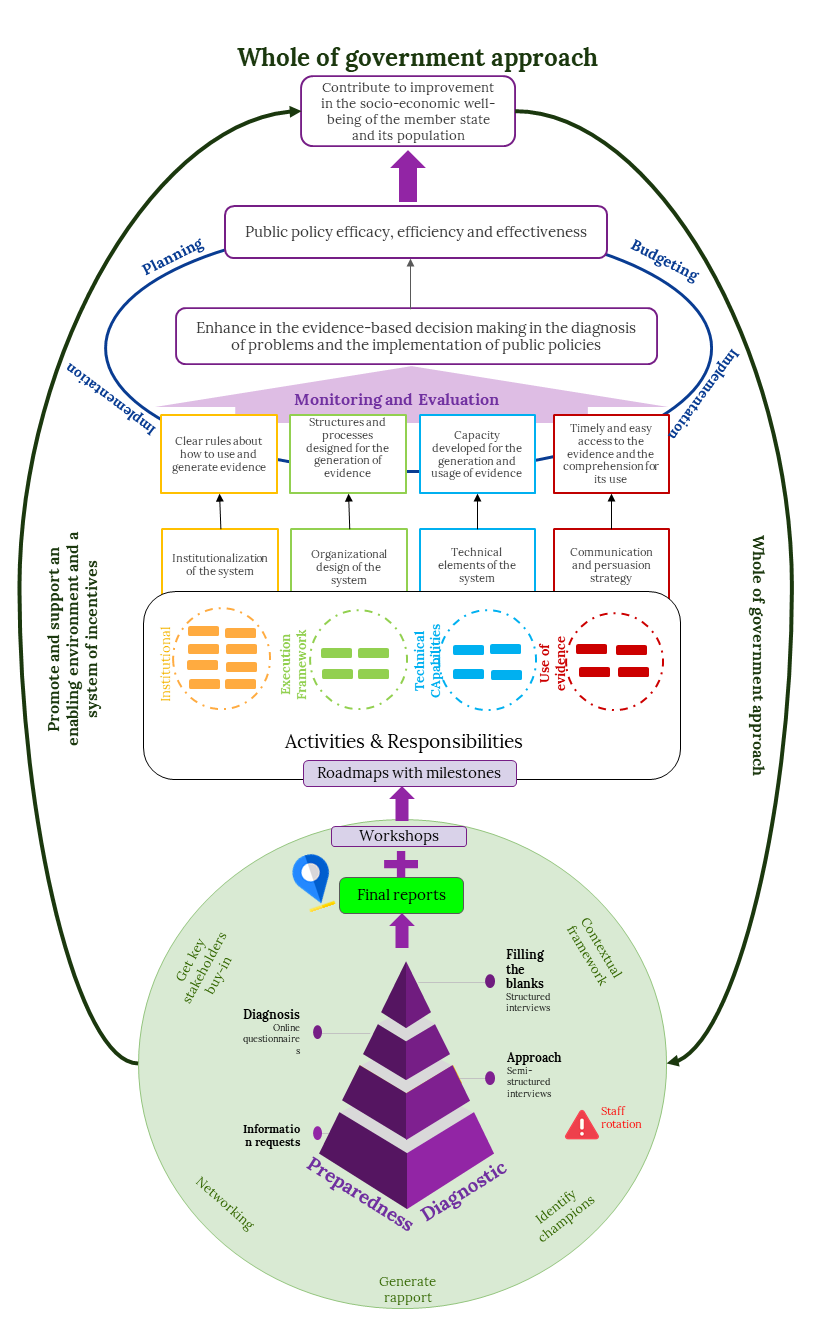
\includegraphics[width=0.75\linewidth]{./images/figure_1} 

}

\caption{Theory of Change}\label{fig:figure1}
\end{figure}

\begin{center}\rule{0.5\linewidth}{0.5pt}\end{center}

As these four dimensions advance and become solid practices, beyond compliance, the system moves towards an increase in evidence-based decision making across government/the institution and across planning, budgeting, and implementation that makes it possible to increase public policies' efficiency, efficacy, and effectiveness.

As the system stays in place and becomes mature, all the dimensions will be strengthened, the enabling environment will advance towards an RBM culture, and all of these will end up contributing to improve the socio-economic well-being of the member state and its population.

\hypertarget{ideal-rbm-system-and-working-process}{%
\section{Ideal RBM system and working process}\label{ideal-rbm-system-and-working-process}}

The development of an RBM System is a complex and nonlinear process that must be contextualized to the specific Member State. To establish a roadmap to strengthen or build an RBM system, the following three elements were considered:

\begin{enumerate}
\def\labelenumi{\arabic{enumi}.}
\tightlist
\item
  A benchmark against which to assess the level of maturity dubbed as ``Ideal RBM System''
\item
  A methodology to obtain general and specific recommendations and,
\item
  A working process and approach to generate ownership
\end{enumerate}

To establish the Ideal RBM system, multiple efforts done over time allow us to learn from experiences in different settings and identify good practices. These good practices represented useful inputs to determine ideal features of an RBM System. The CLEAR LAC team engaged in this collaboration defined four dimensions of an ideal sustainable RBM system (see \protect\hyperlink{fig:figure2}{Figure 2}):

\begin{center}\rule{0.5\linewidth}{0.5pt}\end{center}

\begin{figure}

{\centering 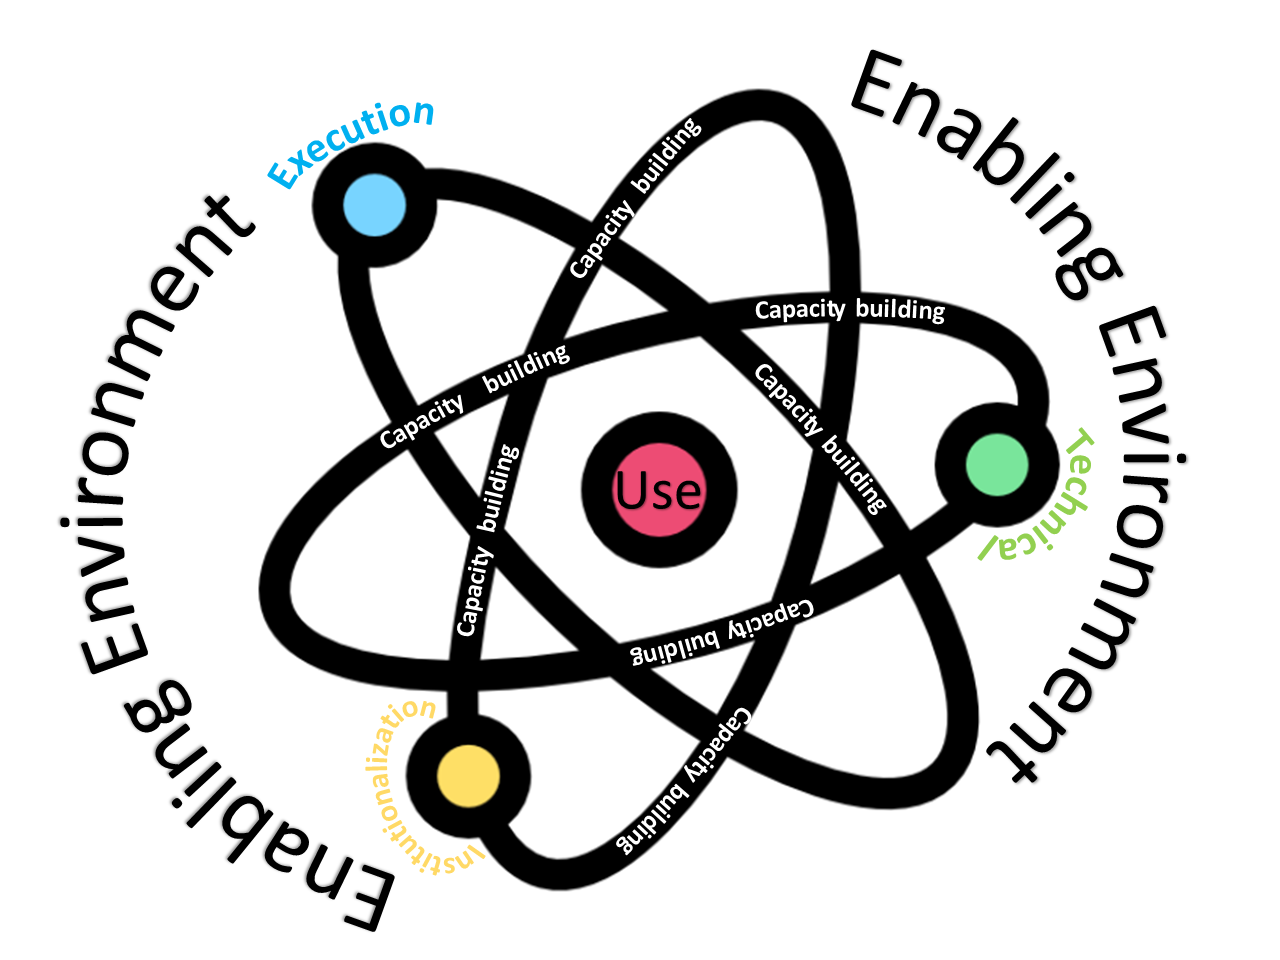
\includegraphics[width=1\linewidth]{./images/figure_2} 

}

\caption{Dimensions of an ideal RBM system}\label{fig:figure2}
\end{figure}

\begin{center}\rule{0.5\linewidth}{0.5pt}\end{center}

\begin{itemize}
\item
  \emph{Institutionalisation:} this dimension focuses on the formal rules that outline the RBM policy in the countries or regional institutions.
\item
  \emph{Execution framework:} this dimension focuses on the systems, resources, processes, methodologies, and tools necessary for the implementation of an RBM system, as well as on the enabling environment.
\item
  \emph{Technical capabilities:} this dimension focuses on the necessary capacities and abilities to implement an RBM System.
\item
  \emph{Use of evidence:} this dimension focuses on the dissemination strategies and incentives aimed at stakeholders with the purpose that they use the evidence generated by the RBM System.
\end{itemize}

Each dimension is integrated by key elements that constitute specific documents, normative frameworks, activities, incentives, among others. These different elements facilitate the operationalisation of the dimension as part of an RBM System. In a third level (beneath dimensions and elements), each element has sub-elements that list their ideal characteristics.

Once all the required information is gathered and analysed (based on the dimension-element-subelement structure) the dimensions will be assessed using a 3-level scale for each sub-element (no, yes, need of improvement)\footnote{For more details on the 3-level scale see \protect\hyperlink{appendixC}{appendix C}} .

For this last step, the progress rate in each sub-element within the element is added end and a cumulative value will be generated to rate the element. Subsequently, all the element values within each dimension are added to determine the progress rate of each dimension.

Finally, the average from the progress of the four dimensions will place each Member State at a specific level of progress (Early initiatives; Committed development; Growing RBM system; Consolidated practices, or Mature state) in the development and implementation of an RBM System (see \protect\hyperlink{appendixC}{Appendix C} for more details).

The working process, defined for this collaboration, identifies Monitoring and Evaluation (M\&E) activities as central elements to be developed and applied in order to affect planning, budgeting, and implementation. \protect\hyperlink{fig:figure3}{Figure 3} presents the working process and highlights the importance of evidence-based decision making (guided and made feasible by M\&E activities and supported, strengthened, and made sustainable through learning and accountability).

\begin{center}\rule{0.5\linewidth}{0.5pt}\end{center}

\begin{figure}

{\centering 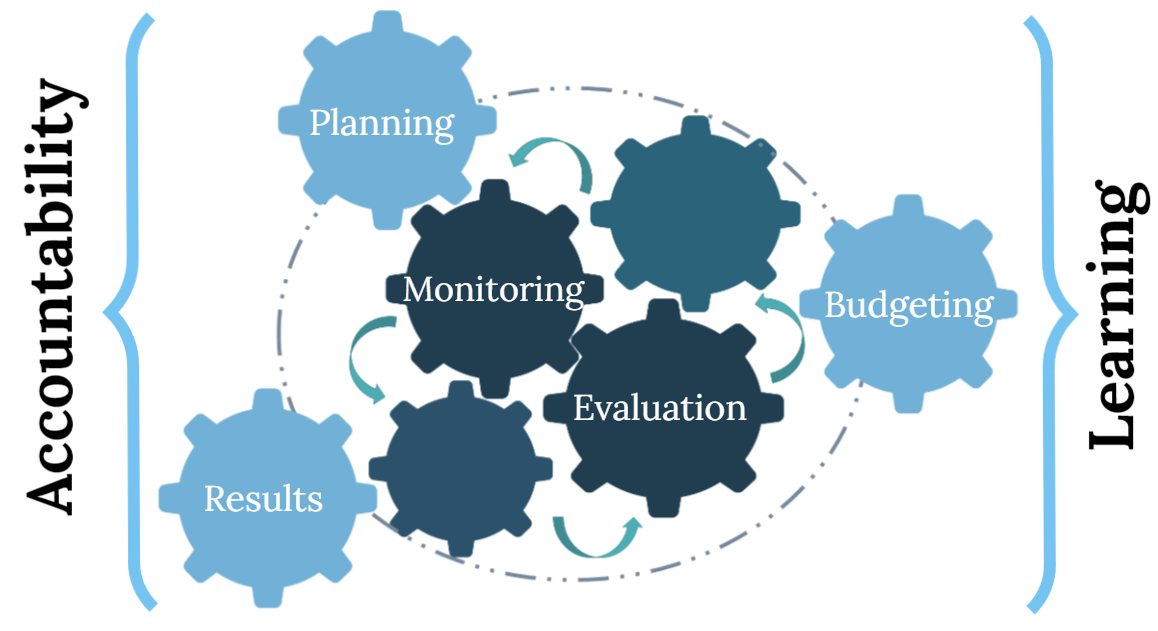
\includegraphics[width=1\linewidth]{./images/figure_3} 

}

\caption{Working Process defined for the CARICOM Collaboration}\label{fig:figure3}
\end{figure}

\begin{center}\rule{0.5\linewidth}{0.5pt}\end{center}

One significant component to strengthen RBM in the Community is to build, in a participatory process, specific roadmaps to continue the development of RBM Systems for each pilot member state and regional institution. The member states and regional institutions participating in the pilot have relevant but heterogeneous advances achieving this goal. To identify these advances, guide the analysis of the Preparedness Diagnostic stages, and develop ownership, the roadmap will be defined in workshops with key stakeholders involved in different levels (management, coordination, and operation).

\hypertarget{stages-of-the-preparedness-diagnostic}{%
\section{Stages of the Preparedness Diagnostic}\label{stages-of-the-preparedness-diagnostic}}

The Preparedness Diagnostic (PD) is a four-stage methodology designed to gain a deep understanding of a Regional Institution's relevant aspects/characteristics when developing an RBM System. One main assumption behind the methodological design of the PD is that building a sustainable RBM System requires the active involvement of multiple stakeholders. The stages of the PD use different data collection methods to identify and engage these stakeholders as well as obtaining information to understand the current policy environment; stakeholder's interests, their roles, motivations, relationship dynamics; map existing institutional structures, practices, and mechanisms; and define capacity building needs.

To have a successful implementation of the PD for this collaboration, the CLEAR LAC team, in coordination with CARICOM Secretariat, selected Executive Coordinators who are representatives for the collaboration from the three Member States (Dominica, Jamaica and Saint Lucia) and the three Regional Institutions (the Caribbean Development Fund, the Caribbean Examinations Council and the CARICOM Implementation Agency for Crime and Security). The role of the Executive Coordinators was key to develop the PD as they have an overall knowledge of their Member State or Regional Institution and have experience in RBM as they have been part of the efforts of their Member State or Regional Institution. As Executive Coordinators for this collaboration they acted as focal points and contributed to identifying and reaching relevant stakeholders in the different stages of the PD and acted as key informants given their experience.

\hypertarget{stages-of-the-pd}{%
\subsection*{Stages of the PD}\label{stages-of-the-pd}}
\addcontentsline{toc}{subsection}{Stages of the PD}

The four stages of the PD (presented in \protect\hyperlink{fig:figure4}{Figure 4} ) are implemented in sequence and personalized based on the findings of the previous stage. They also involve the participation of different stakeholders to obtain a broad perspective of the pilot Member States and Regional Institutions. Below, a brief description of the stages is presented and how they were implemented with the pilots.

\begin{center}\rule{0.5\linewidth}{0.5pt}\end{center}

\begin{figure}

{\centering 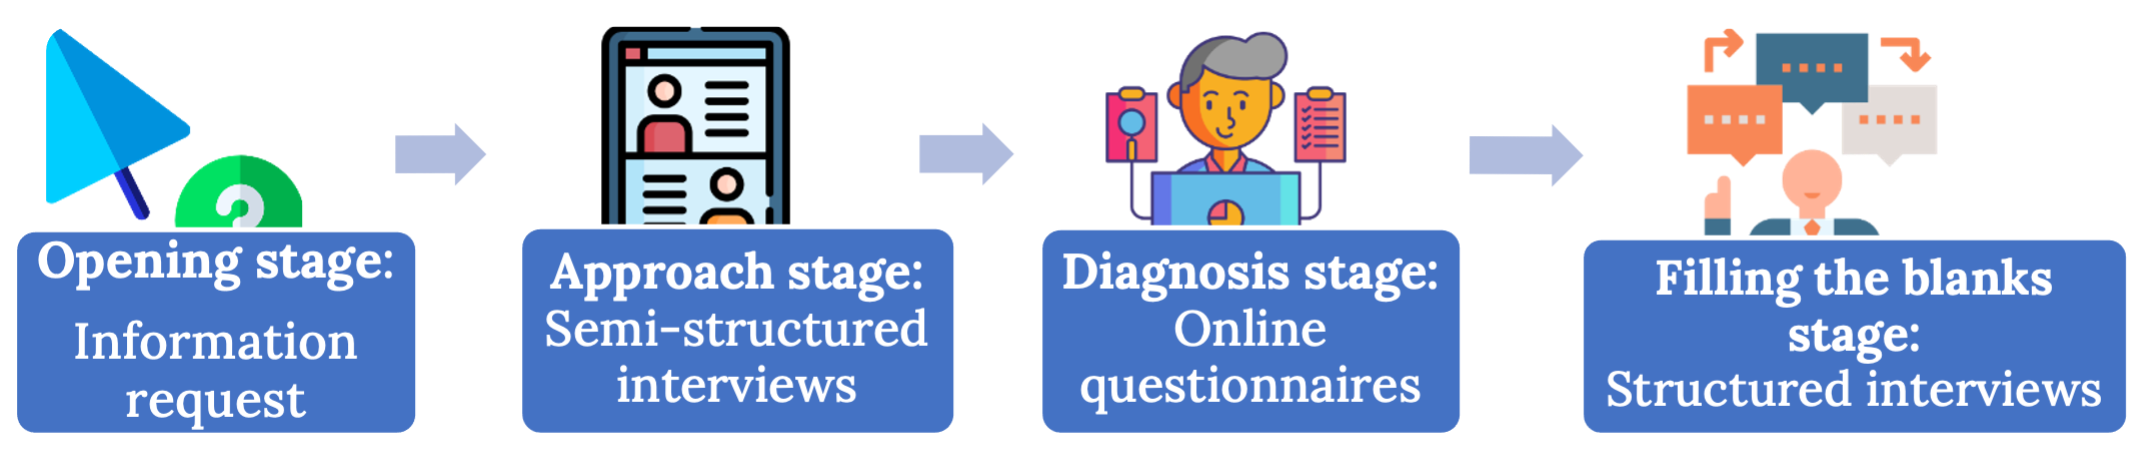
\includegraphics[width=1\linewidth]{./images/figure_4} 

}

\caption{Stages of the Preparedness Diagnostic}\label{fig:figure4}
\end{figure}

\begin{center}\rule{0.5\linewidth}{0.5pt}\end{center}

The \textbf{Opening stage} consisted of a request for different documents from the Executive Coordinators, regarding the pilots' planning, budgeting, and M\&E practices. The desk review and analysis of these documents, in addition to other publicly available information, allowed the design of targeted customized questions for each pilot in the next stage.

The \textbf{Approach stage} involved the identification of various key stakeholders with the support of the Executive Coordinators and the CARICOM Secretariat. The semi-structured interviews addressed general themes that allowed the team to develop rapport with relevant actors within the pilots, as well as obtain additional information about the pilots' current policy environment.

The \textbf{Diagnosis stage} consisted of a series of online questionnaires for the Ministries, Agencies, and Departments of Member States, and Units of Regional Institutions. This stage aimed to gather more in-depth information which would complement information gathered in previous stages and to strengthen the whole of government approach for RBM. The participants were able to respond to questions and upload documents in a timeframe of approximately four weeks, as well as consult with other stakeholders for any additional information within their pilot Member States or Regional Institutions.

Finally, the \textbf{Filling-the-blanks} was aimed at addressing information gaps from the previous stages through a series of structured interviews. This stage targeted other stakeholders such as members of Parliament, representatives of multilateral international organizations, development partners, etc.

\begin{longtable}[]{@{}
  >{\raggedright\arraybackslash}p{(\columnwidth - 4\tabcolsep) * \real{0.1957}}
  >{\centering\arraybackslash}p{(\columnwidth - 4\tabcolsep) * \real{0.3261}}
  >{\raggedleft\arraybackslash}p{(\columnwidth - 4\tabcolsep) * \real{0.4783}}@{}}
\caption{\label{tab:table1} CXC®'s Preparedness Diagnostic Numbers}\tabularnewline
\toprule
\endhead
& \textbf{Stage 1 -- Opening} & Information request to Executive Coordinator + document analysis (+10 documents) + research on official websites. \\
& \textbf{Stage 2 -- Approach} & 4 semi-structured interviews were conducted by the CLEAR LAC team with relevant stakeholders \\
& \textbf{Stage 3 -- Diagnosis} & +5 online questionnaires were sent to MDAs and were answered with both the whole-of-institutional approach \\

\includegraphics{./images/tb1_4.png} & \textbf{Stage 4 -- Filling the blanks} & No structured interviews were conducted by the CLEAR LAC team. \\
\bottomrule
\end{longtable}

All the information gathered in the four stages was systematized and analysed to present the findings in this document.

\hypertarget{strengths-of-the-pd}{%
\subsection*{Strengths of the PD}\label{strengths-of-the-pd}}
\addcontentsline{toc}{subsection}{Strengths of the PD}

\begin{itemize}
\item
  Different stages designed to identify specific stakeholders and to generate rapport with them.
\item
  As the stages are implemented and analysed sequentially, different layers of information are gathered
\item
  Participatory process that leads to the Member States or RI's ownership of the collaboration
\item
  Qualitative and quantitative mixed methods used
\item
  All stages are adapted for to consider the context of each Member State or RI
\end{itemize}

\hypertarget{limitations-of-the-pd}{%
\subsection*{Limitations of the PD}\label{limitations-of-the-pd}}
\addcontentsline{toc}{subsection}{Limitations of the PD}

\begin{itemize}
\item
  Specific results for one pilot cannot be generalized to others given the customization of the instruments and contextual differences among them
\item
  There are time limitations due to tight agendas of stakeholders that complicates reaching all the desired informants.
\item
  All stages were implemented remotely, and it is preferred to have some face-to-face contact with the stakeholders in at least one of the stages to generate rapport
\item
  The duration of the PD is approximately six effective months; however this was extended due to the whole of government/institution approach and the stakeholders' agendas.
\end{itemize}

\hypertarget{section4}{%
\chapter{CXC®'s profile}\label{section4}}

The Caribbean Examination Council (CXC®) is an examination board active since 1972 under an agreement by 15 Commonwealth Caribbean countries (Agreement by the Participating Governments in the Caribbean Community (CARICOM)). The organization was formed with the aim of transforming education in the Caribbean at a time when British examination boards were the leading examination bodies but also when countries in the region were asserting themselves as independent states or advocating for independence, therefore the necessity for internal regional examinations was born to shape future development.

As of today, the Council has 16 English-speaking participating countries and three Dutch-speaking territories that offer examinations. The two main offices of the Council are the Headquarters or Eastern Zone Office (EZO) in Barbados and the Western Zone Office (WZO) in Jamaica.

CXC® provides examinations and certifications for secondary and post-secondary candidates in Caribbean countries in a variety of subjects in academic, technical, and vocational areas. The organization works with educators across the Caribbean who work in sixth form schools, community, state, and teacher-training colleges and universities, as well as specialists from the private sector.

CXC® also uses its expertise and technologies to provide assistance and consultancy services such as the development of syllabuses, preparation and administration of national examinations, training in school-based assessment, item writing, and other aspects of measurement and evaluation, analysis and preparation of reports of students' performance, and preparation of resource materials for both the public and private sector across the region.

The vision of the institution is to be a digitally transformed enterprise that provides quality, relevant, and globally recognised educational services and its mission is to develop the human capital of Caribbean people through partnerships for global competitiveness.

The structure of the Council currently consists of the Vice-Chancellor of the University of West Indies, the Vice-Chancellor of the University of Guyana, three representatives of the University of West Indies, one representative of the University of Guyana, two representatives appointed by each of the Participating Governments (Barbados, Jamaica, Guyana and Trinidad and Tobago), one representative appointed by each of the other Participating Governments, and one representative of the teaching profession appointed by each National Committee from among its members. Members of the Council hold office for a period of three years and Chairmanship is held by one of the Vice-Chancellors or their representatives. The council meets annually to decide on policy framework, and this is carried out by the Administrative and Finance Committee (AFC), the School Examinations Committee (SEC), and its Sub-Committee (SUBSEC).

Other stakeholders are also important to support the organization and its mandates. At the national level, these stakeholders include Ministries of Education, CXC® National Committees, national education authorities, schools, post-secondary and tertiary education institutions, and employers. At the regional level, the stakeholders are the CARICOM Secretariat, OECS Commission, the Caribbean Development Bank, The University of the West Indies, Regional accreditation agencies, the Caribbean Union of Teachers, and regional commercial and employer bodies. Finally, at the international level, these include international development partners such as UNESCO, UNECLAC, UNICEF, UN-WEF, COL, IADB, EU and OAS, international universities and colleges, international examinations and assessment bodies, as well as international qualifications authorities and accreditation agencies and international awarding bodies.

\hypertarget{cxcs-rbm-profile}{%
\section{CXC®'s RBM profile}\label{cxcs-rbm-profile}}

CXC® is considered an advanced results-oriented organisation among CARICOM's Regional Institutions. As the regional examinations board, improving performance with learning is in its essence. It is an institution that, like many others, faces different challenges such as scarce resources, the COVID-19 pandemic, and a constant need to adapt to the changing needs of its customers. To face these challenges and keep delivering services of excellence in the region, CXC® has made relevant efforts into the adoption of an RBM System.

In 2020, CXC® created the Corporate Planning and Strategy Management Unit (CPSM). This unit oversees the institutional planning activities as well as the monitoring and evaluation of the implementation of the strategics' medium-term plan. The development of CXC®'s Strategic Plan 2021 -- 2025, a bold plan intended to guide the institution's initiatives considering the regional needs with a global perspective, is another big step toward a systematic results-oriented approach. The Strategic Plan sets a clear general goal, becoming a globally recognized and top technological educational service provider, and 13 specific strategies to achieve this. All strategies have at least one key performance indicator (KPI), yearly targets, and responsible units or departments.

Another significant advance by CXC® was the adoption of the Spider Impact Software (SIS), a management tool that uses the Balance Scorecard methodology (BSC) to monitor the institution's performance and keep track of the achievement of defined goals. The information captured by the system brings a deep insight into how the initiatives are performing, the budget expenditure, and how much on track CXC® is; and the analysis of this information allows to learn and improve performance. On the road to developing the institutional RBM System, CXC® is committed and motivated to continue the journey.

\hypertarget{section5}{%
\chapter{Main findings}\label{section5}}

As mentioned above, this Preparedness Diagnostic uses a four dimensions analysis as reference. Each dimension contains elements considered relevant to have an ``Ideal RBM System''. This Ideal RBM System serves as a benchmark that allows to compare the current situation in CXC® in relation to the best possible scenario regarding practices, uses and results of RBM. Figure 5 shows the degree of progress that CXC® has in each of the dimensions of analysis, with respect to the ideal scenario.

The elements and sub-elements of the reference Ideal RBM System are not usually part of the status quo, they should be identified, designed, and developed; following this, an institution that has not considered adopting RBM practices would probably not comply or show advances in any of the analysed elements. In this sense, all the advances identified in this diagnosis represent a valuable progress.

It is important to mention that, although there is a numerical value for each dimension, behind the numbers there was a qualitative analysis that determined the current situation of CXC® regarding RBM. Furthermore, these ``ratings'' are in terms of the ideal scenario, so in no way does it represent an outright success or failure, but rather an approximation to the best possible situation of the RBM.

\begin{longtable}[]{@{}
  >{\raggedright\arraybackslash}p{(\columnwidth - 2\tabcolsep) * \real{0.3889}}
  >{\raggedright\arraybackslash}p{(\columnwidth - 2\tabcolsep) * \real{0.3472}}@{}}
\toprule
\begin{minipage}[b]{\linewidth}\raggedright
DIMENSION
\end{minipage} & \begin{minipage}[b]{\linewidth}\raggedright
LEVEL OF PROGRESS
\end{minipage} \\
\midrule
\endhead
INSTITUTIONALISATION & 71\% \\
EXECUTION FRAMEWORK & 46\% \\
TECHNICAL CAPABILITIES & 63\% \\
USE OF EVIDENCE & 43\% \\
\bottomrule
\end{longtable}

\begin{figure}

{\centering 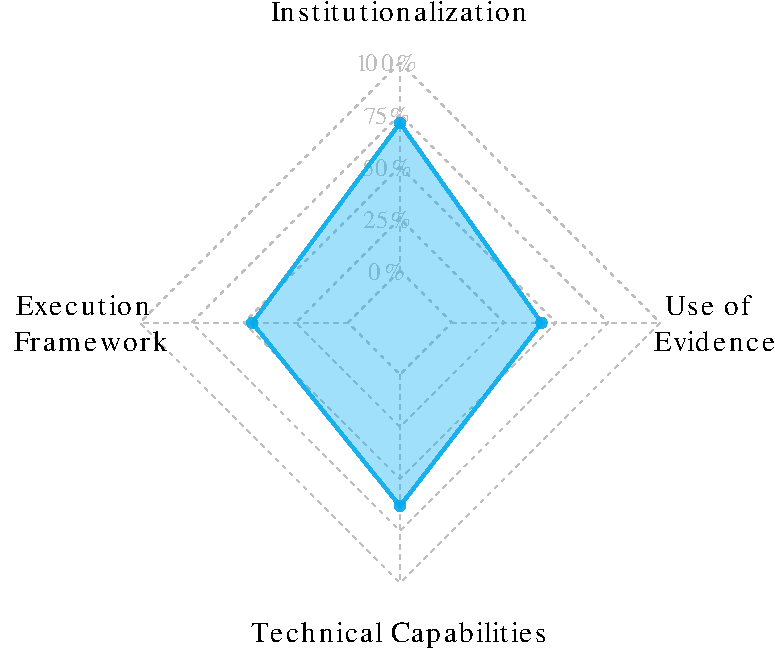
\includegraphics[width=0.7\linewidth]{_main_files/figure-latex/figure5-1} 

}

\caption{Level of progress of the Ideal RBM System}\label{fig:figure5}
\end{figure}

Considering this degree of progress, a metric was built to progressively identify five levels of maturity of RBM systems. In this way, the progress levels presented above are averaged to identify the RBM level in which CXC® is currently located\footnote{ For more information, please see \protect\hyperlink{appendixC}{appendix C}.}. The 5 levels are:

\begin{enumerate}
\def\labelenumi{\arabic{enumi}.}
\tightlist
\item
  Early initiatives
\item
  Committed development
\item
  RBM System
\item
  Consolidated practices
\item
  Mature State
\end{enumerate}

Considering the results in the Preparedness Diagnostic analysis, CXC® is currently in a Growing RBM System level. Significant efforts have been done in developing and implementing a medium-term results-oriented plan with clear strategies, KPIs and yearly targets to track the progress in achieving them. There are also significant efforts in monitoring activities with the use of the BSC methodology in an integrated system (SIS). Also, the Strategic Management mentions an evaluation process that consists in the analysis of the monitoring results, as well as its communication to different stakeholders within the institution to guide decision making. The development of an RBM Policy is still in progress; however, there is a lack of stablished guidelines for M\&E activities with clear activities and responsibilities.

\hypertarget{results-by-dimension}{%
\section{Results by dimension}\label{results-by-dimension}}

The results of this diagnosis for each of the dimensions analysed (and their ideal elements) are presented below in a synthetic manner. For more detailed information on each dimension, elements, and sub-elements, please see \protect\hyperlink{appendixB}{appendix B} and visit the interactive platform with all the disaggregated findings of this PD.

\hypertarget{institutionalisation}{%
\subsection{Institutionalisation}\label{institutionalisation}}

\textbf{Key Message:}
CXC® has clear regulations on planning and M\&E (specifically on strategic evaluation). There are important advances in the development of an RBM policy with the Strategic Management Framework (SMF); In addition, they are working on a new Corporate Performance Framework that will complement the SMF. However, there is no link between the budget process and the use of M\&E results to improve it.

\begingroup\fontsize{12}{14}\selectfont

\begin{tabu} to \linewidth {>{\raggedright}X>{\raggedright}X}
\hline
Ideal Element & Main results/findings\\
\hline
\textbf{1. There is a documented, approved, and binding RBM Policy within the Regional Institution (RI) or a CARICOM RBM general policy for all RIs} & CXC® has been working in a Strategic Management Framework (SMF), a document that contains different elements of an RBM policy. This document is still to be approved.\\
\hline
\textbf{2. There are guidelines that establish the rules and processes to perform monitoring activities:} & The SMF outlines a general monitoring process. Also, CXC® has defined key performance indicators (KPIs) and initiatives that are tracked periodically. However, there are no specific guidelines for monitoring activities.\\
\hline
\textbf{3. There are guidelines that establish the rules and processes to perform evaluation activities:} & The SMF outlines a general evaluation process. However, there are no specific guidelines for performing evaluation activities.\\
\hline
\textbf{4. There are guidelines that establish the rules and processes to address and use of M\&E results} & The SMF mentions that periodic status reports and Management review meetings will be held to discuss the achievement of the strategy through a review of key performance indicators (KPIs) accomplishments.\\
\hline
\textbf{5. There are actions towards building an enabling environment} & The Strategy Evaluation process in the SMF involves periodic meetings with relevant stakeholders from different departments and units within CXC® to discuss the achievement of KPIs and take necessary actions to keep CXC® in the road of accomplishing the targets and objectives in the Strategic Plan 2021 – 2025 (SP).\\
\hline
\textbf{6. There is an institutional Results Oriented Plan defined for a given period:} & CXC® has the SP, a document with strategic objectives, specific initiatives and KPIs, as well as responsible stakeholders. It was developed by the CPSM unit in a participatory process. Its progress is monitored with the  Spider Impact Software (SIS), a strategy and KPI management tool.\\
\hline
\textbf{7. There is an institutional budgeting strategy for a given period:} & CXC® has a three-year budgeting strategy plus a two-year forecast. The SIS generates information that helps guide the budgetary process; however, it is perceived as complete.\\
\hline
\textbf{8. There is a specific unit / department within the Regional Institution responsible for the planning functions:} & The Corporate Planning and Strategy Management Unit oversees coordinating the planning activities in CXC®. This unit ensures collaboration in planning among different departments and divisions.\\
\hline
\textbf{9. There is a specific unit / department within the Regional Institution responsible for the budgeting functions} & The Finance and Office Management Department is responsible for budgeting activities in CXC®; it operates with a financial controller who leads a financial office management team. It oversees implementing and coordinating the budgeting activities within CXC®.\\
\hline
\textbf{10. There is a specific unit / department within the Regional Institution responsible for the M\&E functions} & The CPSM unit is also in charge of implementing and coordinating the M\&E activities in CXC®, such as the management of the SIS, which uses the BSC methodology for strategy management.\\
\hline
\end{tabu}
\endgroup{}

\hypertarget{execution-framework}{%
\subsection{Execution Framework}\label{execution-framework}}

\textbf{Key Message:}
CXC® has strong monitoring practices, uses monitoring tools such as the BSC, and integrates the information in the Spider Impact System to follow-up the institution's performance. It also performs assessments of the KPIs to derive recommendations. However, there is a lack of use-oriented M\&E activities for budgeting.

\begingroup\fontsize{12}{14}\selectfont

\begin{tabu} to \linewidth {>{\raggedright}X>{\raggedright}X}
\hline
Ideal Element & Main results/findings\\
\hline
\textbf{11. There are operative handbooks to implement the monitoring functions (i.e. Logic Framework)} & CXC® uses the BSC methodology to perform its monitoring activities. However, there are no available operative handbooks to implement the monitoring functions within CXC®.\\
\hline
\textbf{12. There are operative handbooks that establish specific steps to develop each stage of the evaluation function} & There are no available operative handbooks to implement the evaluation functions within CXC®.\\
\hline
\textbf{13. The RI collects information to monitor its performance} & The CPSM unit collects information to monitor CXC®s performance using the SIS. The CPSM unit has clear key performance indicators (KPIs) and the initiatives surrounding those objectives. The KPIs’ data is captured on the initiative’s performance, budget spending, issues, and CXC®’s target. After the information is captured, the units/departments analyze it.\\
\hline
\textbf{14. The regional institution has an evaluation plan for its activities, interventions or programs} & CXC® has an evaluation process that consists in the periodic and systematic analysis of the monitoring results.\\
\hline
\end{tabu}
\endgroup{}

\hypertarget{technical-capabilities}{%
\subsection{Technical capabilities}\label{technical-capabilities}}

\textbf{Key Message:}
There are strong capabilities in planning, budgeting, and monitoring activities in CXC®. It is also reported that some staff have received training in evaluation types. However, CXC®'s evaluation needs are not clearly identified.

\begingroup\fontsize{12}{14}\selectfont

\begin{tabu} to \linewidth {>{\raggedright}X>{\raggedright}X}
\hline
Ideal Element & Main results/findings\\
\hline
\textbf{15. There are skilled personnel in the RI with technical capacity and competencies to conduct planning and budgeting for results} & During the development of the Strategic Plan, some staff from different departments was involved in the planning activities to develop capacities. \\
\hline
\textbf{16. There are skilled personnel in the RI with technical capacity and competencies to conduct monitoring activities} & There are certified staff in the Balance Scorecard Institute and indicator development. Also, there has been different training to use the  Spider Impact Software.\\
\hline
\textbf{17. There are skilled personnel in the RI with technical capacity and competencies to conduct evaluations and evaluation activities:} & There are staff with training in evaluation types, but there is lack of training in how to conduct and use the results of evaluations.\\
\hline
\end{tabu}
\endgroup{}

\hypertarget{use-of-evidence}{%
\subsection{Use of evidence}\label{use-of-evidence}}

\textbf{Key Message:}
There is transparency in planning, and annual reports were delivered until 2019. In addition, there are mechanisms for the use of M\&E results to improve planning and partially for budgeting. However, there is no transparency with budgeting. A strategy to generate a culture of evidence use is not identified.

\begingroup\fontsize{12}{14}\selectfont

\begin{tabu} to \linewidth {>{\raggedright}X>{\raggedright}X}
\hline
Ideal Element & Main results/findings\\
\hline
\textbf{18. RBM documents are publicly available for consultation} & There are some publicly available documents such as the Strategic Plan 2021 – 2025 and annual reports. However, budget reports are not available for public consultation.\\
\hline
\textbf{19. There are guidelines that establish the rules and processes to address and use of M\&E results} & The Strategic Management Framework has specific processes for monitoring and evaluation activities, and the final element of the processes is to deliver status reports and hold Management Review Meetings. The expected result of the meetings is to act in case the defined targets are not being achieved.\\
\hline
\textbf{20. M\&E results are systematically included in the planning \& budgeting of programs and public policies} & The Corporate Planning and Strategy Management Unit produces progress reports in the implementation of CXC®’s Strategic Plan and Corporate Performance Reports. These reports are directed to the Internal - Line and Senior Management and Executive.\\
\hline
\textbf{21. The RI has mechanisms to measure the use of evidence that the RBM system generates} & The use of the  Spider Impact Software allows CXC® to track its progress in the achievement of defined targets. Also, the recommendations from monitoring information analysis and the Management Review Meetings allow for adjustments to be made. However, it is not clear if there are mechanisms to measure the use of this analysis and recommendations.\\
\hline
\end{tabu}
\endgroup{}

\hypertarget{main-challenges-to-strengthen-the-rbm-system}{%
\section{Main challenges to strengthen the RBM system}\label{main-challenges-to-strengthen-the-rbm-system}}

As mentioned in \protect\hyperlink{section2}{section 2.2}, the development of an RBM System is a complex, nonlinear, and continuous process that must be contextualized in each country. In doing so, it is important to consider the main challenges that Dominica faces when it comes to strengthening its RBM system. This diagnosis identifies three major challenges:

1.Changing the culture and fostering the enabling environment to have an RBM system in place implies a change of mindset of public servants at all levels. It should be considered that throughout the process there must be a constant awareness/sensitization strategy, both in the short and mid-term, that allows public servants to identify why it is important to have this mindset change in pursuit of RBM. In other words, in a constant way, remember why RBM is important and how it can improve performance and lives.

\begin{enumerate}
\def\labelenumi{\arabic{enumi}.}
\setcounter{enumi}{1}
\item
  Since this collaboration has a whole-of-institution approach, it is necessary to have a top-bottom commitment in which leaders and decision-makers show the benefits of the RBM system through actions that consider the evidence derived from the system. This means that we need a top-bottom approach to use, and thereby demonstrate its usefulness, the information and evidence derived from the RBM system to improve planning and budgeting decisions.
\item
  For the RBM system to be sustainable, it is of the utmost importance to generate a system of incentives and ensure that there is a balance between positive and negative incentives (such as potential penalties for non-compliance), to keep the system moving forward. The positive incentives can take different forms, from monetary to symbolic, such as the delivery of awards and recognition for good performance in public service.
\end{enumerate}

\hypertarget{section6}{%
\chapter{Next steps to building the roadmap}\label{section6}}

RBM entails more than just abiding with certain requirements. Compliance is just not enough; it has to do with a change of mindset about the way things are done. This change of mindset involves different areas and moments of the administration. Having reviewed the main results from the preparedness diagnostic in terms of the dimensions of elements considered as part of an ideal RBM system, this section introduces the next steps that will be carried out as part of the process of building contextualized roadmaps.

The roadmap will present paths to influence planning, budgeting, implementation, and the M\&E functions, as well as accountability and learning promotion. The main objective is for CXC® to have a defined action course that also specifies responsibilities and shows the importance of the participation of all relevant stakeholders.

\begin{center}\rule{0.5\linewidth}{0.5pt}\end{center}

\begin{figure}

{\centering 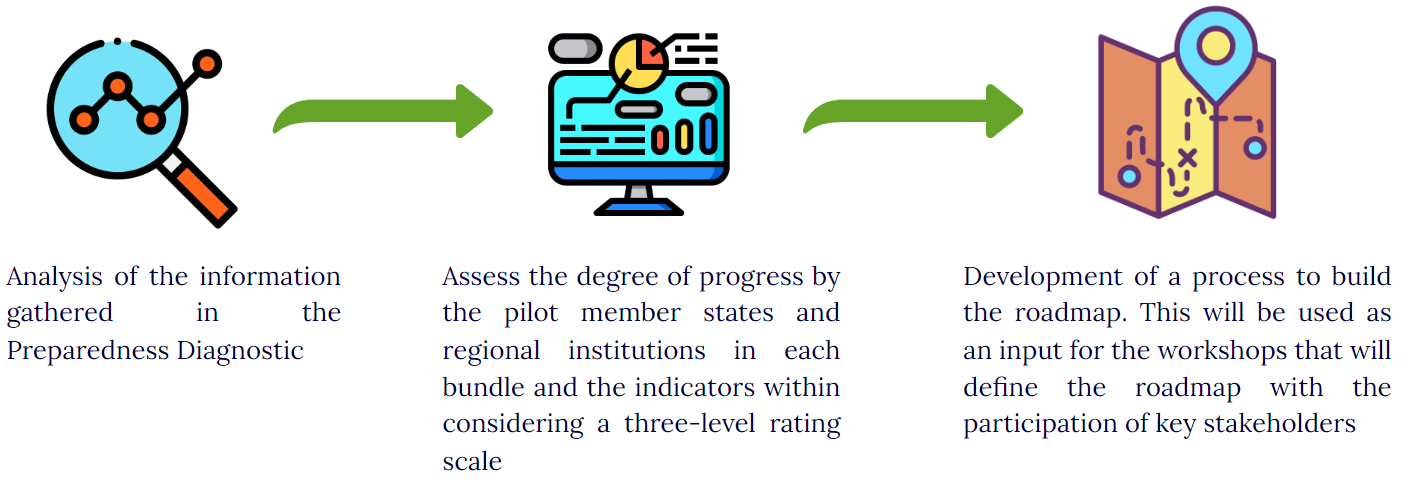
\includegraphics[width=1\linewidth]{./images/figure_6} 

}

\caption{From an ideal RBM system to the roadmaps}\label{fig:figure6}
\end{figure}

\begin{center}\rule{0.5\linewidth}{0.5pt}\end{center}

The whole process has a coproduction approach, were aside of the CLEAR LAC team, the CARICOM Secretariat, and the Executive Coordinators, key stakeholders will be involved in a fluid process to develop a learning loop that provides feedback and improves the process.
***

\begin{figure}

{\centering 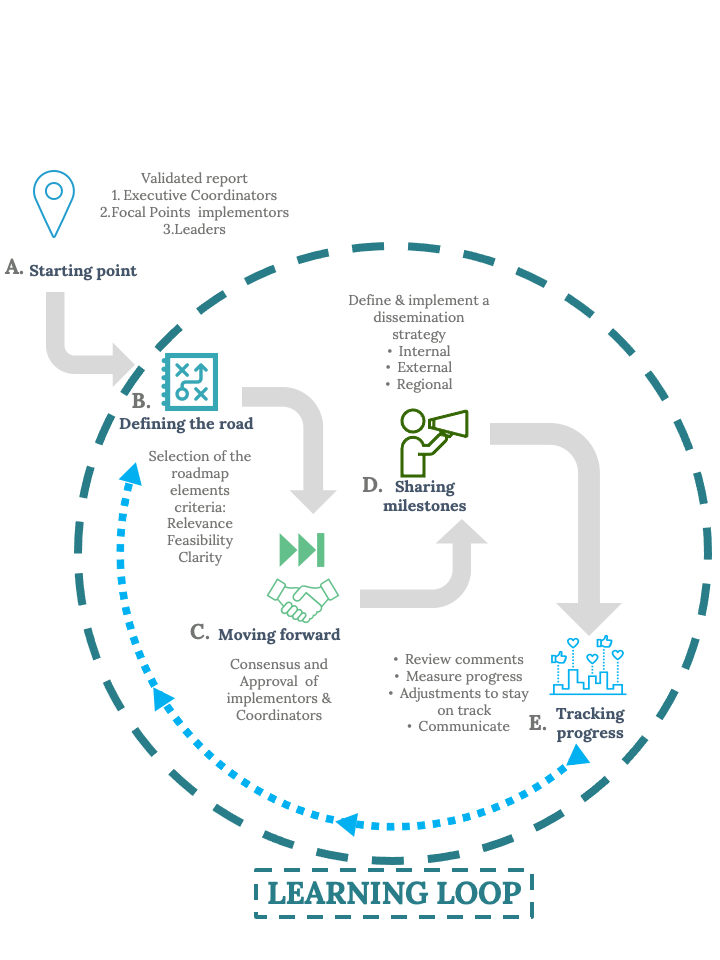
\includegraphics[width=0.75\linewidth]{./images/figure_7} 

}

\caption{Learning loop}\label{fig:figure7}
\end{figure}

\begin{center}\rule{0.5\linewidth}{0.5pt}\end{center}

This report is considered as the \emph{starting point} in this process; take into consideration that, as \protect\hyperlink{fig:figure7}{figure 7} illustrates, the process started before its publication.

Once the first draft was completed, it will be shared with key stakeholders for review and validation, starting with the Executive Coordinators. Once the feedback period concluded, the report itself became an input for what is to come and will be distributed with multiple purposes (including generating knowledge, aiding in empowering key stakeholders in the path of strengthening RBM practices, and promoting appropriation of the next steps).

The next steps start with \emph{defining the road}, engaging key stakeholders to coproduce contextualized mid-term roadmaps that will include specific activities and milestones that sought to materialize their implementation. To develop the roadmap, the CLEAR LAC team has designed a series of workshops with the participation of stakeholders involved in the different areas and levels of what is to be the national RBM system, and that have been carefully identified as part of the Preparedness Diagnostic process.

To \emph{move forward}, this first draft of the roadmap is presented to other relevant stakeholders to build a consensus and support for the process. It is crucial to gain whole-of-government ownership, so it is important to define and implement a dissemination strategy for \emph{sharing clearly define milestones} in different levels: internal, external, and regional once they have been clearly defined and responsibilities have been assigned. Finally, it is important to \emph{track the progress} of implementation and communicate results to assure that the Member State learns from the process, adjusts, and stays on the recommended path, as well as communicating results. The continuum process of identifying, sharing, reviewing, and adjusting represents a learning loop.

\hypertarget{stakeholders-contribution-analysis}{%
\section{Stakeholders' contribution analysis}\label{stakeholders-contribution-analysis}}

This section presents an analysis of stakeholders to identify which of them are relevant to strengthening the RBM system. Each of these actors has different levels of decision and execution. A proposal of their possible contribution to improve the system and generate the necessary evidence to improve decision-making regarding planning, budgeting and thus achieve the expected results of CXC® is presented here based on the CLEAR LAC's team analysis considering their positions and experience.

The analysis is summarized in the following table . During the roadmap development workshops that will be held with institution's stakeholders, new stakeholders could be identified or some of those presented here could be discarded. Once its RBM Policy is approved and published, we will be able to have greater clarity on the roles, responsibilities, capacities, and relevance of the stakeholders that will integrate the system in a whole-of-institutional approach.

\begin{table}

\caption{\label{tab:unnamed-chunk-8}Stakeholders’ contribution analysis}
\centering
\fontsize{12}{14}\selectfont
\begin{tabu} to \linewidth {>{\raggedright}X>{\raggedright}X>{\raggedright}X}
\hline
Stakeholder / Position & Responsibilities / Role in the system & Incentives to be part of the system\\
\hline
\textbf{Administrative and Finance Committee (AFC)} & •Define M\&E information needs & •Achieve better results for CXC®\\
\hline
\textbf{} & •Demand for M\&E information to guide decision-making & •Provide better educational services to the regional citizens\\
\hline
\textbf{CARICOM Secretariat} & •Demand better results from CXC®, as well as transparency and accountability & •Achieve regional objectives in terms of educational services provided to the region citizens\\
\hline
\textbf{} & •Develop incentives for the good performance of CXC® and the rest of Regional Institutions & \\
\hline
\textbf{} & •Create a best RBM practice repository and disseminate them among the Regional Institutions & \\
\hline
\textbf{Citizens} & •Demand better services from CXC® & •Not Applicable\\
\hline
\textbf{Corporate Planning and Strategy Management Unit (CPSM)} & •Coordinate the operationalisation of CXC®’s RBM System & •Achieve the targets defined in the Strategic Plan 2021 – 2025\\
\hline
\textbf{} & •Coordinate the implementation of the Strategic Plan 2021 – 2025 & •CXC®’s RBM System as an example among the Regional Institutions\\
\hline
\textbf{} & •Gather the specific M\&E needs from CXC®’s different departments to guide planning, budgeting and implementation activities & \\
\hline
\textbf{} & •Undertake CXC®’s M\&E activities & \\
\hline
\textbf{} &  \vphantom{1} & \\
\hline
\textbf{Director of Corporate Services} & •Define the M\&E universe for CXC® (what information is needed, who needs it, when is it needed and for what purpose) & •Achieve the targets defined in the Strategic Plan 2021 – 2025\\
\hline
\textbf{} & •Define, direct and supervise the M\&E processes and incentives to use the M\&E results & •CXC®’s RBM System as an example among the Regional Institutions\\
\hline
\textbf{} & •Define the M\&E annual program and identify clear responsibilities & \\
\hline
\textbf{} & •Supervise the implementation of the M\&E activities and provide recommendations to the M\&E process & \\
\hline
\textbf{} & •Follow-up the implementation of the roadmap & \\
\hline
\textbf{} & •Present reports to the AFC and CXC®’s Registrar and Pro-Registrar regarding the progress on the roadmap implementation & \\
\hline
\textbf{Registrar \& Pro-Registrar} & •Instruct the necessary actions to implement CXC®’s RBM Policy \& System & •Achieve better results for CXC®\\
\hline
\textbf{} & • Provide policy direction with respect to the development of the RBM with a whole-of-institutional approach & •Provide better educational services to the regional citizens •Get more resources for their institutions\\
\hline
\textbf{} & • Disseminate the RBM strategy to the public & •Be recognized for good performance\\
\hline
\textbf{}\textbf{} &  & •Become the leaders of the sectors in which they operate\\
\hline
\textbf{Units \& Departments} & •Communicate M\&E needs (what information is needed, when is it needed and for what) & •Access to pertinent and timely information to guide decision making\\
\hline
\textbf{} & • Use the results of M\&E activities to guide planning, budgeting and implementation activities & \\
\hline
\textbf{} & •Provide recommendations regarding the M\&E process & \\
\hline
\textbf{Universities} & •Use the results of the M\&E processes & •Offer RBM/M\&E training to Regional Institutions (increase earnings and strengthening the community of practice in the region)\\
\hline
\textbf{} & •Participate in the M\&E processes of CXC® \vphantom{1} & \\
\hline
\textbf{} & •Offer M\&E services both in training and monitoring and evaluating \vphantom{1} & \\
\hline
\textbf{} & •Demand evidence derived from M\&E \vphantom{1} & \\
\hline
 &  & \\
\hline
\textbf{VOPE (CaribbeanEvaluators International)} & •Use the results of the M\&E processes & •Offer RBM/M\&E training to Regional Institutions (increase earnings and strengthening the community of practice in the region)\\
\hline
\textbf{} & •Participate in the M\&E processes of CXC® & \\
\hline
\textbf{} & •Offer M\&E services both in training and monitoring and evaluating & \\
\hline
\textbf{} & •Demand evidence derived from M\&E & \\
\hline
\multicolumn{3}{l}{\rule{0pt}{1em}\textit{Note: }}\\
\multicolumn{3}{l}{\rule{0pt}{1em}Developed by the CLEAR LAC technical team in charge of the collaboration}\\
\end{tabu}
\end{table}

\hypertarget{references-sources}{%
\chapter*{References \& Sources}\label{references-sources}}
\addcontentsline{toc}{chapter}{References \& Sources}

\begin{itemize}
\tightlist
\item
  CXC® / Education / Examinations / Certifications. (2021, August 31st). Caribbean Examinations Council. \url{https://CXC}®.org
\end{itemize}

\hypertarget{appendix-appendix}{%
\appendix}


\hypertarget{appendixA}{%
\chapter{Conceptual framework (CLEAR LAC)}\label{appendixA}}

\hypertarget{key-dimensions-of-a-sustainable-rbm-system}{%
\section{Key dimensions of a sustainable RBM System}\label{key-dimensions-of-a-sustainable-rbm-system}}

The development of an RBM System is a complex and nonlinear process that must be contextualized to the specific region, country, or regional institution. However, the multiple efforts done over time allow us to learn from experiences in different settings and identify good practices. These good practices represent useful inputs to be considered when embarked on this road.

One significant component to strengthen RBM in the Community is to build, in a participatory process, specific roadmaps to continue the development of RBM Systems for each pilot member state and regional institution. The member states and regional institutions participating in the pilot have significant but heterogeneous advances achieving this goal. To identify these advances and guide the analysis of the Preparedness Diagnostic stages, the CLEAR LAC team defined four dimensions of an ideal and sustainable RBM System:

\begin{itemize}
\item
  \emph{Institutionalisation:} this dimension focuses on the formal rules that defines, outlines and formalize the RBM Systems in the countries.
\item
  \emph{Execution framework:} this dimension focuses on the systems, resources, processes, methodologies, and tools necessary for the implementation of the RBM system, as well as incentives that promote an enabling environment.
\item
  \emph{Technical capabilities:} this dimension focuses on the capacities, abilities, and resources necessary to implement and sustain the RBM System.
\item
  \emph{Use of evidence:} this dimension focuses on the dissemination strategies and incentives aimed at stakeholders with the purpose that they use the evidence generated by the RBM System and its measurement.
\end{itemize}

\hypertarget{ideal-elements-sub-elements}{%
\section{Ideal elements \& sub-elements}\label{ideal-elements-sub-elements}}

The four dimensions previously mentioned were conceptualized as necessary components when building an operating and sustainable RBM system. To have a better understanding of what the progress in each dimension entails, we propose a set of ideal elements and sub-elements taken from different contexts and experiences where they have been successfully implemented or recommended. Each dimension has a set of elements that represent activities, documents, normative frameworks, skills, incentives, etc.; and every element has a set of sub-elements that describe the ideal characteristics of the element. The sub-elements allow to translate concepts into practice, and, after gathering and analysing information, this knowledge can be translated into specific actions.

Unlike the dimensions, as RBM Systems are designed and built considering contextual factors, some elements and sub-elements should be taken as a guide as different contexts will result in variations on their interpretation and level of relevance/priorities. This framework allows for adaptations, recognizing that every context is particular and that there is no unique checklist that may apply to all contexts.

\begin{table}
\centering
\begin{tabular}[t]{l}
\hline
I. Institutionalisation Ideal elements\\
\hline
\multicolumn{1}{l}{\textbf{1. There is a documented, approved, and binding RBM Policy within the CXC®.}}\\
\hline
\hspace{1em}1.1 It outlines guiding principles / pillars that are aligned to a results-oriented approach\\
\hline
\hspace{1em}1.2 It communicates what RBM entails (e.g., clear definitions for key concepts) and clearly states how it works\\
\hline
\hspace{1em}1.3 It identifies key actors who are responsible for the coordination and the measurement of the overall results of the RBM policy\\
\hline
\hspace{1em}1.4 It identifies key actors who are responsible for supervising the implementation of the RBM policy and their functions\\
\hline
\hspace{1em}1.5 It is use-oriented in planning, budgeting, and implementing towards results, transparency and accountability\\
\hline
\hspace{1em}1.6 The funding for M\&E activities and the responsible are identified\\
\hline
\multicolumn{1}{l}{\textbf{2. There are guidelines that establish the rules and processes to perform monitoring activities}}\\
\hline
\hspace{1em}2.1 They identify indicator types and the dimensions they want to measure (e.g. efficiency, efficacy), and monitoring tools (e.g. logic framework) to be developed for each project / social programme\\
\hline
\hspace{1em}2.2 They identify specific timeframes to collect indicator data and develop monitoring tools to measure the indicators (e.g., collect every six months) for each project\\
\hline
\hspace{1em}2.3 They have criteria to ensure data collection quality (design, measurement, report)\\
\hline
\hspace{1em}2.4 They integrate the indicators as a monitoring system\\
\hline
\hspace{1em}2.5 The monitoring system has a stablished process to update its information periodically\\
\hline
\hspace{1em}2.6 The monitoring system has a stablished process to update its indicators periodically\\
\hline
\hspace{1em}2.7 There are rules providing all parts in the monitoring process with a way of presenting their opinion (e.g., institutional positions)\\
\hline
\multicolumn{1}{l}{\textbf{3. There are guidelines that establish the rules and processes to perform evaluation activities}}\\
\hline
\hspace{1em}3.1 They identify key stakeholders to be part of the evaluation process (e.g., evaluation process coordinators, evaluation subjects, evaluation process implementors)\\
\hline
\hspace{1em}3.2 They identify specific evaluation types\\
\hline
\hspace{1em}3.3 The identify specific timeframes for each evaluation type\\
\hline
\hspace{1em}3.4 They identify specific characteristics and functions of evaluators\\
\hline
\hspace{1em}3.5 It establishes an iterative process of evaluation (e.g.,  is not a one-time exercise)\\
\hline
\hspace{1em}3.6 They identify the elements to be included in the evaluation's ToRs (e.g., objectives of the evaluation, the role and responsibilities of the evaluator and evaluation client and the resources available to conduct the evaluation)\\
\hline
\hspace{1em}3.7 They outline the operationalization process of the institution’s evaluation agenda (e.g., it is agreed among relevant stakeholders)\\
\hline
\hspace{1em}3.8 There have quality control mechanisms for evaluation activities (e.g., quality attribute listings, quality evaluations, peer review, satisfaction surveys, evaluate the evaluator)\\
\hline
\hspace{1em}3.9 There are rules providing all parts in the evaluation process with a way of presenting their opinion (e.g., institutional position)\\
\hline
\multicolumn{1}{l}{\textbf{4. There are guidelines that establish the rules and processes to address and use M\&E results}}\\
\hline
\hspace{1em}4.1 They identify instruments to measure the RBM System results\\
\hline
\hspace{1em}4.2 They identify mechanisms to use monitoring results\\
\hline
\hspace{1em}4.3 They identify mechanisms to use evaluation results\\
\hline
\hspace{1em}4.4 They establish rules and processes that require the budgeting process to consider the results of M\&E activities (they make explicit the link between planning and budgeting)\\
\hline
\multicolumn{1}{l}{\textbf{5. There are formal actions towards building an enabling environment}}\\
\hline
\hspace{1em}\hspace{1em}5.1 There are key stakeholders identified as responsible for these formal actions\\
\hline
\hspace{1em}\hspace{1em}5.2 There are strategies to enhance or attenuate positive or negative incentives for the use of monitoring\\
\hline
\hspace{1em}5.3 There are strategies to enhance or attenuate positive or negative incentives for the use of evaluation\\
\hline
\hspace{1em}5.4 There are mechanisms for the participation of stakeholders in the definition of monitoring activities and needs\\
\hline
\hspace{1em}5.5 There are mechanisms for the participation of stakeholders in the definition of evaluation activities and needs\\
\hline
\hspace{1em}5.6 There are periodic meetings involving relevant stakeholders to review the M\&E information as an RBM System feedback exercise\\
\hline
\hspace{1em}5.7 There is a permanent strategy to communicate and sensitize about the benefits and challenges of M\&E\\
\hline
\multicolumn{1}{l}{\textbf{6. There is an institutional Results Oriented Plan defined for a given period:}}\\
\hline
\hspace{1em}6.1 It has defined objectives\\
\hline
\hspace{1em}6.2 It is constructed in a participatory process\\
\hline
\hspace{1em}6.3 It is constructed using the information generated by the RBM System\\
\hline
\hspace{1em}6.4 It has defined strategies to implement the plan\\
\hline
\hspace{1em}6.5 It has defined indicators and monitoring tools by mandate, and they measure outcomes and outputs\\
\hline
\hspace{1em}6.6 It is evaluated by mandate\\
\hline
\hspace{1em}6.7 It has specific evaluation activities\\
\hline
\hspace{1em}6.8 It has defined responsible actors\\
\hline
\hspace{1em}6.9 It considers regional (CARICOM) objectives\\
\hline
\multicolumn{1}{l}{\textbf{7. There is an institutional budgeting strategy for a given period :}}\\
\hline
\hspace{1em}7.1 It is allocated according to the objectives/goals/activities of the institutional planning\\
\hline
\hspace{1em}7.2 It considers the prioritization of the objectives/goals/activities identified in the institutional planning\\
\hline
\hspace{1em}7.3 It is allocated using the information generated by evidence and the RBM System\\
\hline
\hspace{1em}7.4 The budget allocation is defined in annual terms (e.g., it specifies the starting date, relevant milestones dates, and the end date)\\
\hline
\hspace{1em}7.5 It stablishes a specific allocation of resources for M\&E activities according to the budget period\\
\hline
\hspace{1em}7.6 It considers other available information to define its allocation (e.g., Member States’ statistics/poverty measurements/etc.)\\
\hline
\hspace{1em}7.7 It considers regional planning, objectives/goals/activities\\
\hline
\hspace{1em}7.8 The key actors and their responsibilities are clearly defined\\
\hline
\multicolumn{1}{l}{\textbf{8. There is a specific unit / department within the Regional Institution responsible for the planning functions:}}\\
\hline
\hspace{1em}8.1 The unit / department has the necessary financial and infrastructural resources to undertake its functions and activities\\
\hline
\hspace{1em}8.2 The unit / department has the necessary human resources to undertake its functions and activities\\
\hline
\hspace{1em}8.3 The unit / department is known by all the other institution's departments and holds regular communication with relevant decision-making actors within the institution\\
\hline
\end{tabular}
\end{table}

\begin{table}
\centering
\begin{tabular}[t]{l}
\hline
II. Excecution Framework Ideal elements\\
\hline
\multicolumn{1}{l}{\textbf{9. There is a specific unit / department within the Regional Institution responsible for the budgeting functions}}\\
\hline
\hspace{1em}9.1 The unit / department has the necessary financial and infrastructural resources to undertake its functions and activities\\
\hline
\hspace{1em}9.2 The unit / department has the necessary human resources to undertake its functions and activities\\
\hline
\hspace{1em}9.3 The unit / department is known by all the other institution's departments and holds regular communication with relevant decision-making actors within the institution\\
\hline
\multicolumn{1}{l}{\textbf{10. There is a specific unit / department within the Regional Institution responsible for the M\&E functions}}\\
\hline
\hspace{1em}10.1 The unit / department has the necessary financial and infrastructural resources to undertake its functions and activities\\
\hline
\hspace{1em}10.2 The unit / department has the necessary human resources to undertake its functions and activities\\
\hline
\hspace{1em}10.3 The unit / department is known by all the other institution's departments and holds regular communication with relevant decision-making actors within the institution\\
\hline
\multicolumn{1}{l}{\textbf{11. There are operative handbooks to implement the monitoring functions (e.g., Logic Framework)}}\\
\hline
\hspace{1em}\hspace{1em}11.1 They identify all the relevant activities to develop each stage of the process (e.g., Specific activities within the analysis of the project's context, stakeholder)\\
\hline
\hspace{1em}\hspace{1em}11.2 They outline specific timeframes to implement every stage of the process\\
\hline
\hspace{1em}11.3 They identify the responsible in every stage of the process\\
\hline
\hspace{1em}11.4 They outline a dissemination strategy of the LF results (what, how, when and to who do you want to diffuse the results)\\
\hline
\hspace{1em}11.5 The indicators are oriented to results and outcomes\\
\hline
\multicolumn{1}{l}{\textbf{12. There are operative handbooks that establish specific steps to develop each stage of the evaluation function}}\\
\hline
\hspace{1em}12.1 They identify all the relevant activities to develop each stage of the evaluation process (e.g., evaluators selection, ToR definition for each evaluation, evaluation supervision)\\
\hline
\hspace{1em}12.2 They outline specific timeframes to implement every stage of the process\\
\hline
\hspace{1em}12.3 They outline a dissemination strategy of the evaluation results (what, how, when and to who do you want to diffuse the results)\\
\hline
\hspace{1em}12.4 They identify the responsible in every stage of the process\\
\hline
\end{tabular}
\end{table}

\begin{table}
\centering
\begin{tabular}[t]{l}
\hline
III. Technical Capabilities Ideal elements\\
\hline
\multicolumn{1}{l}{\textbf{13. The RI collects information to monitor its performance:}}\\
\hline
\hspace{1em}13.1 It is timely: it is available when making policy decisions\\
\hline
\hspace{1em}13.2 It is trustworthy: there is a validation mechanism.\\
\hline
\hspace{1em}13.3 It is systematized: it is organized for easy understanding.\\
\hline
\hspace{1em}13.4 It is relevant regarding its management: it allows to measure the indicators of planning and budgeting for results.\\
\hline
\hspace{1em}13.5 It has a defined update period\\
\hline
\hspace{1em}13.6 It is monitored periodically within the time horizon of planning and budgeting for results.\\
\hline
\hspace{1em}13.7 It is replicable: anyone with access to the information may obtain the same results.\\
\hline
\hspace{1em}13.8 It is collected considering vulnerable populations (e.g., they measure the access of women/indigenous/disabled people to the institution’s interventions, they measure improvements in the goal to achieve gender equality). Please provide examples of gender approach strategies considered by your institution.\\
\hline
\hspace{1em}13.9 It is public/accessible to citizens.\\
\hline
\hspace{1em}13.10 It is analyzed in periodic reports\\
\hline
\hspace{1em}13.11 It is documented in a user-friendly way (simple, concise, and easy-to-use decision-making reports).\\
\hline
\hspace{1em}13.12 It considers the Performance Measurement Framework (CARICOM´s monitoring tool for the Strategic Plan)\\
\hline
\hspace{1em}13.13 The regional institution reports its monitoring results in the CARMES web portal\\
\hline
\multicolumn{1}{l}{\textbf{14. The regional institution has an evaluation plan for its activities, interventions or programs:}}\\
\hline
\hspace{1em}14.1 It has a specific evaluation strategy for a given period.\\
\hline
\hspace{1em}14.2 It has evaluation activities delegated to specific actors (e.g. institution's M\&E unit, external agencies)\\
\hline
\hspace{1em}14.3 It is the result of institutionalized planning exercises; that is, it follows an established procedure.\\
\hline
\hspace{1em}14.4 It is known by those responsible for the areas/units of the institution.\\
\hline
\hspace{1em}14.5 It has established the activities, interventions or programs to evaluate.\\
\hline
\hspace{1em}14.6 It is designed considering vulnerable populations approach (e.g., the evaluations involve gender analytical tools and methodologies, etc.).\\
\hline
\hspace{1em}14.7 The document is public/accessible to citizens.\\
\hline
\multicolumn{1}{l}{\textbf{15. There are skilled personnel in CXC® with technical capacity and competencies to conduct planning and budgeting for results}}\\
\hline
\hspace{1em}15.1 They have technical skills to use derived evidence from M\&E to improve planning (identify priorities, vulnerable population, what works to attend that priorities)\\
\hline
\hspace{1em}15.2 They have competencies to use M\&E results to define results-oriented budgeting (e.g., identify priorities, new public problems that should be addressed, policies that work, compare between policies), as well as soft skills\\
\hline
\hspace{1em}15.3 They have competencies to coordinate with other with other institutions and relevant actors\\
\hline
\multicolumn{1}{l}{\textbf{16. There are skilled personnel in the RI with technical capacity and competencies to conduct monitoring activities}}\\
\hline
\hspace{1em}16.1 They have technical skills to collect indicator data\\
\hline
\hspace{1em}16.2 They have technical skills to use monitoring tools\\
\hline
\hspace{1em}16.3 They have the competences to identify monitoring needs in order to collect relevant, pertinent and timely data\\
\hline
\end{tabular}
\end{table}

\begin{table}
\centering
\begin{tabular}[t]{l}
\hline
IV. Use of Evidence Ideal elements\\
\hline
\multicolumn{1}{l}{\textbf{17. There are skilled personnel in the RI with technical capacity and competencies to conduct evaluations and evaluation activities}}\\
\hline
\hspace{1em}17.1 They have the competences to perform different evaluation types (e.g., design, process, impact) and use different methodologies (e.g., quantitative, qualitative, mixed methods)\\
\hline
\hspace{1em}17.2 They have the competences to identify evaluation needs and match them with proper evaluation types and methodologies: define evaluation horizon and ask relevant evaluation questions\\
\hline
\hspace{1em}17.3 They have the competences to formulate reports that include relevant, pertinent, and timely information for different stakeholders\\
\hline
\hspace{1em}17.4 There is a capacity strengthening plan for on-going training in RBM and M\&E\\
\hline
\multicolumn{1}{l}{\textbf{18. RBM documents and the RIs performance information are publicly available for consultation}}\\
\hline
\hspace{1em}\hspace{1em}18.1 Institutional planning documents are publicly available\\
\hline
\hspace{1em}18.2 Institutional budget plans are publicly available\\
\hline
\hspace{1em}18.3 Documents that mention the results/findings/recommendations of monitoring and evaluation activities are publicly available\\
\hline
\hspace{1em}18.4 M\&E manuals / guidelines /ToRs are publicly available\\
\hline
18.5 There is a dissemination strategy of evidence about the institution’s performance targeted to different stakeholders (e.g., citizens, CARICOM, decision-makers, private sector, NGOs)\\
\hline
\multicolumn{1}{l}{\textbf{19. There is an enabling environment for the use of M\&E results}}\\
\hline
\hspace{1em}19.1 There are explicit positive or negative incentives for the use of monitoring results\\
\hline
\hspace{1em}19.2 There are explicit positive or negative incentives for the use of evaluation results\\
\hline
\hspace{1em}19.3 There are knowledge management practices\\
\hline
\multicolumn{1}{l}{\textbf{20. M\&E results are systematically included in the planning and budgeting}}\\
\hline
\hspace{1em}\hspace{1em}20.1 They are used in an institutionalized way: they follow a established procedure\\
\hline
\hspace{1em}\hspace{1em}20.2 There are action plans or other management instruments to ensure M\&E results/recommendations are implemented\\
\hline
\hspace{1em}\hspace{1em}20.3 They identify the target population of institutional interventions\\
\hline
\hspace{1em}\hspace{1em}20.4 They identify general and specific recommendations to improve the implementation of institutional interventions\\
\hline
\hspace{1em}\hspace{1em}20.5 They inform the design/redesign of institutional interventions\\
\hline
\hspace{1em}\hspace{1em}20.6 They inform the initial budget allocations of institutional interventions\\
\hline
\hspace{1em}20.7 They inform the budget increase/decrease/suspension of institutional interventions\\
\hline
\hspace{1em}20.8 Evaluation findings/reports are updated periodically\\
\hline
20.9 The M\&E results are used to define the RIs budget\\
\hline
\multicolumn{1}{l}{\textbf{21. CXC® has mechanisms to measure the use of the evidence that the RBM system generates}}\\
\hline
\hspace{1em}21.1 There are mechanisms to know how much the reports and publications on M\&E are downloaded or used by citizens\\
\hline
\hspace{1em}21.2 There are use-of-evidence measurements to improve the use of M\&E results strategy\\
\hline
\end{tabular}
\end{table}

\hypertarget{levels-of-progress}{%
\section{Levels of progress}\label{levels-of-progress}}

The Preparedness Diagnostic methodology is designed to gain a deep understanding of a country or institution's relevant aspects/characteristics when developing an RBM System. The different stages are meant to gather information from different stakeholders to achieve a whole of government / institutional outlook. The dimensions with ideal elements and sub-elements guide the analysis of the information gathered in order to identify the level of progress of a specific government or institution.

The scale used to assess the sub-elements are:

\begin{itemize}
\tightlist
\item
  \textbf{No:} there is no documented advance in the sub-element
\item
  \textbf{Needs improvement:} there is documented advance in the sub-element, but do not cover all the criteria express in the sub-element.
\item
  \textbf{Yes:} there is documented proof that the sub-element complies with the needed/ideal characteristics
\end{itemize}

Each scale level has an assigned value, and every element will have a result obtained from the total sum of its sub-element's scores. The average score of the elements per dimension results in the dimension's score, and the average score of the four dimensions will place the Member state/regional Institution in one of the following \textbf{levels of progress} of their RBM Systems:

\begin{itemize}
\tightlist
\item
  Level 0. No RBM
\item
  Level 1. Early initiatives: there are some initiatives to develop RBM-related structures and focus on monitoring activities
\item
  Level 2. Committed development: there are RBM-related structures being stablished and limited evaluation activities
\item
  Level 3.. Growing RBM system: there are RBM-related structures being stablished and limited evaluation activities
\item
  Level 4. Consolidated practices: there are integrated efforts (political will, capacity building and some whole-of-government consensus) to develop the RBM System
\item
  Level 5. Mature state: Functioning and sustainable RBM System in place that generates credible, reliable and timely information that improves public policies
\end{itemize}

\begin{center}\rule{0.5\linewidth}{0.5pt}\end{center}

\begin{figure}

{\centering 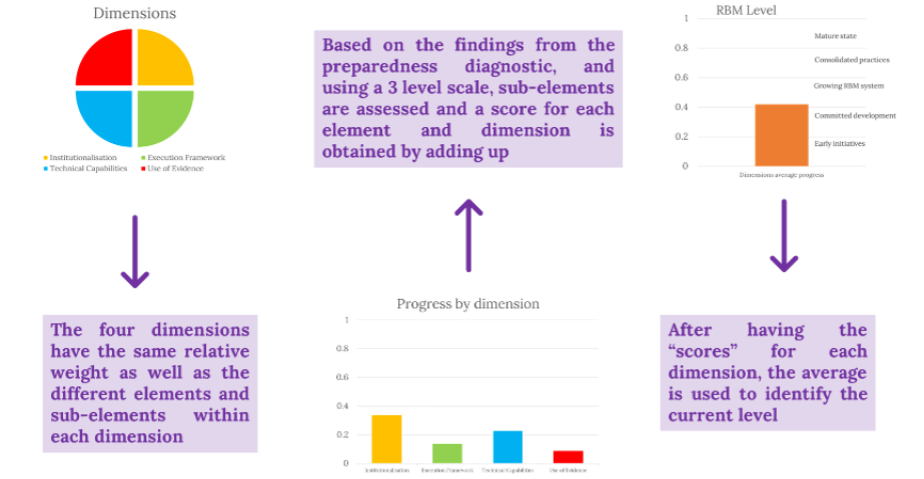
\includegraphics[width=1\linewidth]{./images/figure_8} 

}

\caption{How to identify the current level of the RBM system maturity}\label{fig:figure8}
\end{figure}

\begin{center}\rule{0.5\linewidth}{0.5pt}\end{center}

\hypertarget{appendixB}{%
\chapter{Detailed findings}\label{appendixB}}

In the following table, you can consult all the findings found in this PD in detail.

\begin{table}
\centering
\begin{tabular}[t]{l|l}
\hline
I. Institutionalisation Detailed Findings &  \\
\hline
\multicolumn{2}{l}{\textbf{1. There is a documented, approved, and binding RBM Policy within the CXC®.}}\\
\hline
\hspace{1em}1.1 It outlines guiding principles / pillars that are aligned to a results-oriented approach & The SMF is being designed as a guide to implement a whole-of-institution strategic management framework to orient CXC®’s policy actions into achieving its strategic goals.\\
\hline
\hspace{1em}1.2 It communicates what RBM entails (e.g., clear definitions for key concepts) and clearly states how it works & There are definitions around the RBM framework such as Balance Scorecard, Key Performance Indicators and SWOT Analysis.\\
\hline
\hspace{1em}1.3 It identifies key actors who are responsible for the coordination and the measurement of the overall results of the RBM policy & There are roles and responsibilities identified, from the oversight and management of the Corporate and Divisional Strategy to CXC®’s staff in charge of executing their assigned initiatives. CXC®’s Senior manager of CPSM is responsible for the monitoring and reporting of the corporate plan, but it is not clear if this position is responsible of measuring the results of the SMF implementation.\\
\hline
\hspace{1em}1.4 It identifies key actors who are responsible for supervising the implementation of the RBM policy and their functions & CXC®’s Senior manager of the CPSM unit is responsible for the monitoring and reporting of the corporate plan, but it is not clear if this position is mandated to supervise the implementation of the SMF.\\
\hline
\hspace{1em}1.5 It is use-oriented in planning, budgeting, and implementing towards results, transparency and accountability & There are some mentions of budget planning and resource allocation; however, there is not a link between M\&E activities and the use of M\&E evidence to improve planning and budgeting,\\
\hline
\hspace{1em}1.6 The funding for M\&E activities and the responsible are identified & The CPSM unit is responsible for the M\&E activities within CXC®. However, there are no mentions of securing M\&E funding.\\
\hline
\multicolumn{2}{l}{\textbf{2. There are guidelines that establish the rules and processes to perform monitoring activities}}\\
\hline
\hspace{1em}2.1 They identify indicator types and the dimensions they want to measure (e.g. efficiency, efficacy), and monitoring tools (e.g. logic framework) to be developed for each project / social programme & CXC® uses the BSC methodology and the  Spider Impact Software (SIS). Also, CXC®s SP sets strategic objectives with clear KPIs and yearly targets. The KPIs are categorized in leading and lagging indicators\\
\hline
\hspace{1em}2.2 They identify specific timeframes to collect indicator data and develop monitoring tools to measure the indicators (e.g., collect every six months) for each project & CXC®’s SP sets strategic objectives with clear KPIs and yearly targets that are measured using the SIS.\\
\hline
\hspace{1em}2.3 They have criteria to ensure data collection quality (design, measurement, report) & Not applicable\\
\hline
\hspace{1em}2.4 They integrate the indicators as a monitoring system & The CPSM unit uses the SIS to monitor CXC®’s performance, budget spending, and target achievements.\\
\hline
\hspace{1em}2.5 The monitoring system has a stablished process to update its information periodically & It was mentioned that the SIS has a stablished process to update its information periodically. The CPSM unit requests for periodically information to different units within CXC®, and this is uploaded in the system.\\
\hline
\hspace{1em}2.6 The monitoring system has a stablished process to update its indicators periodically & It was mentioned that the SIS updates its indicators periodically.\\
\hline
\hspace{1em}2.7 There are rules providing all parts in the monitoring process with a way of presenting their opinion (e.g., institutional positions) & There is no evidence of rules providing all parts in the monitoring process with a way of presenting their opinion\\
\hline
\multicolumn{2}{l}{\textbf{3. There are guidelines that establish the rules and processes to perform evaluation activities}}\\
\hline
\hspace{1em}3.1 They identify key stakeholders to be part of the evaluation process (e.g., evaluation process coordinators, evaluation subjects, evaluation process implementors) & The SMF identified stakeholders and units to be part of the evaluation process such as the CPSM unit, Senior Managers of CXC®,  the Director of Corporate Services (DCS) and the Executive Management Committee (EMC).\\
\hline
\hspace{1em}3.2 They identify specific evaluation types & Not applicable\\
\hline
\hspace{1em}3.3 The identify specific timeframes for each evaluation type & Not applicable\\
\hline
\hspace{1em}3.4 They identify specific characteristics and functions of evaluators & Not applicable\\
\hline
\hspace{1em}3.5 It establishes an iterative process of evaluation (e.g.,  is not a one-time exercise) & The evaluation process in the SMF is said to be established in a regular basis.\\
\hline
\hspace{1em}3.6 They identify the elements to be included in the evaluation's ToRs (e.g., objectives of the evaluation, the role and responsibilities of the evaluator and evaluation client and the resources available to conduct the evaluation) & Not applicable\\
\hline
\hspace{1em}3.7 They outline the operationalization process of the institution’s evaluation agenda (e.g., it is agreed among relevant stakeholders) & The process in the SMF established steps for the Strategy Evaluation and involves relevant stakeholders.\\
\hline
\hspace{1em}3.8 There have quality control mechanisms for evaluation activities (e.g., quality attribute listings, quality evaluations, peer review, satisfaction surveys, evaluate the evaluator) & Not applicable\\
\hline
\hspace{1em}3.9 There are rules providing all parts in the evaluation process with a way of presenting their opinion (e.g., institutional position) & Not applicable\\
\hline
\multicolumn{2}{l}{\textbf{4. There are guidelines that establish the rules and processes to address and use M\&E results}}\\
\hline
\hspace{1em}4.1 They identify instruments to measure the RBM System results & The evaluation process mentions the use of the BSC methodology and the SIS to measure whether the objectives identified in the SP were achieved or not.\\
\hline
\hspace{1em}4.2 They identify mechanisms to use monitoring results & The SMF mentions that periodic status reports and management review meetings will be held to review monitoring results,   to drive organizational focus and to correct potential issues.\\
\hline
\hspace{1em}4.3 They identify mechanisms to use evaluation results & The evaluation process mentions that periodic status reports and management review meetings will be held to review the analysis of KPI achievements, to drive organizational focus and to correct potential issues.\\
\hline
\hspace{1em}4.4 They establish rules and processes that require the budgeting process to consider the results of M\&E activities (they make explicit the link between planning and budgeting) & After analysing the gathered information, it was identified that there are other needs on M\&E results to inform the budgeting process that are not met.\\
\hline
\multicolumn{2}{l}{\textbf{5. There are formal actions towards building an enabling environment}}\\
\hline
\hspace{1em}\hspace{1em}5.1 There are key stakeholders identified as responsible for these formal actions & Specific units and stakeholders are identified such as the CPSM unit, Senior Managers of CXC®,  the Director of Corporate Services (DCS) and the Executive Management Committee (EMC).\\
\hline
\hspace{1em}\hspace{1em}5.2 There are strategies to enhance or attenuate positive or negative incentives for the use of monitoring & It was mentioned that the BSC is cascaded down the organization and also, the SIS  allows the staff to know if their performance is achieving the expected results.\\
\hline
\hspace{1em}5.3 There are strategies to enhance or attenuate positive or negative incentives for the use of evaluation & Not applicable\\
\hline
\hspace{1em}5.4 There are mechanisms for the participation of stakeholders in the definition of monitoring activities and needs & There is no evidence of mechanisms for the participation of stakeholders in the definition of monitoring activities and needs.\\
\hline
\hspace{1em}5.5 There are mechanisms for the participation of stakeholders in the definition of evaluation activities and needs & There is no evidence of mechanisms for the participation of stakeholders in the definition of monitoring activities and needs.\\
\hline
\hspace{1em}5.6 There are periodic meetings involving relevant stakeholders to review the M\&E information as an RBM System feedback exercise & Not applicable\\
\hline
\hspace{1em}5.7 There is a permanent strategy to communicate and sensitize about the benefits and challenges of M\&E & Not applicable\\
\hline
\multicolumn{2}{l}{\textbf{6. There is an institutional Results Oriented Plan defined for a given period:}}\\
\hline
\hspace{1em}6.1 It has defined objectives & The SP has 13 strategic objectives categorized in 4 strategic themes: Customer \& Stakeholder Excellence, Technology \& Innovation Excellence, Operational Excellence, and Governance Excellence.\\
\hline
\hspace{1em}6.2 It is constructed in a participatory process & The SP was constructed in a participatory process, involving staff from different units.\\
\hline
\hspace{1em}6.3 It is constructed using the information generated by the RBM System & The SP was developed with the monitoring information gathered by CXC®.\\
\hline
\hspace{1em}6.4 It has defined strategies to implement the plan & Each strategic objective has specific initiatives and initiatives descriptions to be implemented in order to achieve them.\\
\hline
\hspace{1em}6.5 It has defined indicators and monitoring tools by mandate, and they measure outcomes and outputs & Each strategic objective has at least one KPI and yearly targets to compare against. These KPIs are monitored with the SIS.\\
\hline
\hspace{1em}6.6 It is evaluated by mandate & The Strategy Evaluation in the SMF presents a process to review and analyse the KPIs achievements. As the SMF is being developed as CXC®s RBM policy, this evaluation process will be a mandate.\\
\hline
\hspace{1em}6.7 It has specific evaluation activities & The Strategic Management Framework outlines a general evaluation process called Strategy Evaluation. This process consists of the periodic review and analysis of the KPIs achievements to identify if the defined objectives were achieved, as well as regular meetings with relevant stakeholders to take necessary actions and ensure the strategy can be achieved.\\
\hline
\hspace{1em}6.8 It has defined responsible actors & The SP has clear strategic objectives with intended results and KPIs. Each strategic objective has an “owner” or responsible. Also, the BSC methodology is cascaded down the organization, so the staff within CXC® has clear responsibilities assigned.\\
\hline
\hspace{1em}6.9 It considers regional (CARICOM) objectives & CXC® has responsibility for the educational development of the Caribbean Human Resource. The planning is based on what CARICOM intends to achieve in education for its member states. Given the nature of the institution, it is essential to coordinate with CARICOM.\\
\hline
\multicolumn{2}{l}{\textbf{7. There is an institutional budgeting strategy for a given period :}}\\
\hline
\hspace{1em}7.1 It is allocated according to the objectives/goals/activities of the institutional planning & There is a link between planning and budgeting as the Finance and Office Management Department (FOMD) develops the budget to accomplish the initiatives in the Strategic Plan.\\
\hline
\hspace{1em}7.2 It considers the prioritization of the objectives/goals/activities identified in the institutional planning & There is a link between planning and budgeting as the Finance and Office Management Department (FOMD) develops the budget to accomplish the initiatives in the Strategic Plan.\\
\hline
\hspace{1em}7.3 It is allocated using the information generated by evidence and the RBM System & The SIS generates information on budget expenditure. However, after analysing the gathered information, it was identified that there are other needs on M\&E results to inform the budgeting process that are not met.\\
\hline
\hspace{1em}7.4 The budget allocation is defined in annual terms (e.g., it specifies the starting date, relevant milestones dates, and the end date) & CXC®’s budget is defined in annual terms for the three-year budgeting strategy plus the two-year forecast.\\
\hline
\hspace{1em}7.5 It stablishes a specific allocation of resources for M\&E activities according to the budget period & The budget establishes a specific allocation of resources for the CPSM unit, as well as for the SIS.\\
\hline
\hspace{1em}7.6 It considers other available information to define its allocation (e.g., Member States’ statistics/poverty measurements/etc.) & It was mentioned that CXC®’s strategies respond to regional needs. however, it is not clear if CXC® uses regional data to define its budget allocation.\\
\hline
\hspace{1em}7.7 It considers regional planning, objectives/goals/activities & It was mentioned that, as a CARICOM’s regional institution, CXC®’s strategies respond to regional needs.\\
\hline
\hspace{1em}7.8 The key actors and their responsibilities are clearly defined & Key actors and their responsibilities are not defined; however, the Ministry of Finance does mid-term fiscal review regarding MDAs budgeting. Each MDA has a financial director and chief financial officer that submit monthly reports.\\
\hline
\multicolumn{2}{l}{\textbf{8. There is a specific unit / department within the Regional Institution responsible for the planning functions:}}\\
\hline
\hspace{1em}8.1 The unit / department has the necessary financial and infrastructural resources to undertake its functions and activities & It was mentioned that, even though there are resource constraints, the CPSM unit has the  necessary financial and infrastructural resources to undertake its functions and activities\\
\hline
\hspace{1em}8.2 The unit / department has the necessary human resources to undertake its functions and activities & The CPSM unit has 3 people on as staff working full time. It was mentioned that a fourth person was joining the unit.\\
\hline
\hspace{1em}8.3 The unit / department is known by all the other institution's departments and holds regular communication with relevant decision-making actors within the institution & The CPSM unit coordinates CXC®’s planning functions and involves the input of different departments and units within CXC®. Due to the SIS, this unit is known by all CXC®.\\
\hline
\end{tabular}
\end{table}

\begin{table}
\centering
\begin{tabular}[t]{l|l}
\hline
II. Excecution Framework Detailed Findings &  \\
\hline
\multicolumn{2}{l}{\textbf{9. There is a specific unit / department within the Regional Institution responsible for the budgeting functions}}\\
\hline
\hspace{1em}9.1 The unit / department has the necessary financial and infrastructural resources to undertake its functions and activities & It was mentioned that, even though there are resource constraints, the FOMD has the  necessary financial and infrastructural resources to undertake its functions and activities\\
\hline
\hspace{1em}9.2 The unit / department has the necessary human resources to undertake its functions and activities & Some KPIs are taken into account in the budget so that they can be tracked identifying how ministries are using their resources to improve outputs related to the KPIs.\\
\hline
\hspace{1em}9.3 The unit / department is known by all the other institution's departments and holds regular communication with relevant decision-making actors within the institution & The head of the FOMD works with all units and departments to derive the budget. All the units within a department are in constant communication about their budget needs.\\
\hline
\multicolumn{2}{l}{\textbf{10. There is a specific unit / department within the Regional Institution responsible for the M\&E functions}}\\
\hline
\hspace{1em}10.1 The unit / department has the necessary financial and infrastructural resources to undertake its functions and activities & It was mentioned that, even though there are resource constraints, the CPSM unit has the  necessary financial and infrastructural resources to undertake its functions and activities\\
\hline
\hspace{1em}10.2 The unit / department has the necessary human resources to undertake its functions and activities & The CPSM unit has 3 people on as staff working full time. It was mentioned that a fourth person was joining the unit.\\
\hline
\hspace{1em}10.3 The unit / department is known by all the other institution's departments and holds regular communication with relevant decision-making actors within the institution & The CPSM unit coordinates CXC®’s the M\&E functions and involves the input of different departments and units within CXC®. Due to the SIS, this unit is known by all CXC®.\\
\hline
\multicolumn{2}{l}{\textbf{11. There are operative handbooks to implement the monitoring functions (e.g., Logic Framework)}}\\
\hline
\hspace{1em}\hspace{1em}11.1 They identify all the relevant activities to develop each stage of the process (e.g., Specific activities within the analysis of the project's context, stakeholder) & Not applicable\\
\hline
\hspace{1em}\hspace{1em}11.2 They outline specific timeframes to implement every stage of the process & Not applicable\\
\hline
\hspace{1em}11.3 They identify the responsible in every stage of the process & Not applicable\\
\hline
\hspace{1em}11.4 They outline a dissemination strategy of the LF results (what, how, when and to who do you want to diffuse the results) & Not applicable\\
\hline
\hspace{1em}11.5 The indicators are oriented to results and outcomes & There are indicators oriented to results and outcomes in the CRRP’s Results Framework. However, there is no evidence that they are being measured in practice.\\
\hline
\multicolumn{2}{l}{\textbf{12. There are operative handbooks that establish specific steps to develop each stage of the evaluation function}}\\
\hline
\hspace{1em}12.1 They identify all the relevant activities to develop each stage of the evaluation process (e.g., evaluators selection, ToR definition for each evaluation, evaluation supervision) & The broad steps of the evaluation process are stated in the Strategy evaluation section of the SMF. However, the specific evaluation activities are not documented.\\
\hline
\hspace{1em}12.2 They outline specific timeframes to implement every stage of the process & Not applicable\\
\hline
\hspace{1em}12.3 They outline a dissemination strategy of the evaluation results (what, how, when and to who do you want to diffuse the results) & The evaluation process mentions that periodic status reports and management review meetings will be held to review the analysis of KPI achievements, to drive organizational focus and to correct potential issues.\\
\hline
\hspace{1em}12.4 They identify the responsible in every stage of the process & The SMF identified stakeholders and units to be part of the evaluation process such as the CPSM unit, Senior Managers of CXC®,  the Director of Corporate Services (DCS) and the Executive Management Committee (EMC).\\
\hline
\end{tabular}
\end{table}

\begin{table}
\centering
\begin{tabular}[t]{l|l}
\hline
III. Technical Capabilities Detailed Findings &  \\
\hline
\multicolumn{2}{l}{\textbf{13. The RI collects information to monitor its performance:}}\\
\hline
\hspace{1em}13.1 It is timely: it is available when making policy decisions & Monthly reports are prepared and sent to different divisions based on the results of the QST. In addition, monthly and quarterly reports are also sent to the registrar, the government body, and the executive management team to assist decision-making. However, after analysing the gathered information, it was identified that information is not that timely for budgeting decisions.\\
\hline
\hspace{1em}13.2 It is trustworthy: there is a validation mechanism. & CPSM uses the balanced scorecard methodology for strategic management. However, it is not clear if there is a validation mechanism.\\
\hline
\hspace{1em}13.3 It is systematized: it is organized for easy understanding. & After analysing that the information can be better organized and systematized for easy understanding.\\
\hline
\hspace{1em}13.4 It is relevant regarding its management: it allows to measure the indicators of planning and budgeting for results. & After analysing the gathered information, it was identified that there are other needs on M\&E results to inform the budgeting process that are not met.\\
\hline
\hspace{1em}13.5 It has a defined update period & It was mentioned that the information is updated periodically.\\
\hline
\hspace{1em}13.6 It is monitored periodically within the time horizon of planning and budgeting for results. & It was mentioned that the KPIs data measuring and collecting period/time data varies. Some are measured monthly, quarterly, semi-annually, and annually, depending on the nature of the KPI.\\
\hline
\hspace{1em}13.7 It is replicable: anyone with access to the information may obtain the same results. & It is not clear if there is a documentation of the formulas needed to estimate the KPIs and yearly targets.\\
\hline
\hspace{1em}13.8 It is collected considering vulnerable populations (e.g., they measure the access of women/indigenous/disabled people to the institution’s interventions, they measure improvements in the goal to achieve gender equality). Please provide examples of gender approach strategies considered by your institution. & It is not clear if CXC® considers specific needs of vulnerable populations.\\
\hline
\hspace{1em}13.9 It is public/accessible to citizens. & The results from the M\&E activities performed by CXC® are not publicly available for citizens.\\
\hline
\hspace{1em}13.10 It is analyzed in periodic reports & There are periodic reports and meetings held to discuss the analysis of the KPIs achievements.\\
\hline
\hspace{1em}13.11 It is documented in a user-friendly way (simple, concise, and easy-to-use decision-making reports). & After analysing that the information can be better documented in a user-friendly way.\\
\hline
\hspace{1em}13.12 It considers the Performance Measurement Framework (CARICOM´s monitoring tool for the Strategic Plan) & CARICOM’s Performance Measurement Framework is not considered in CXC®’s monitoring activities.\\
\hline
\hspace{1em}13.13 The regional institution reports its monitoring results in the CARMES web portal & It was mentioned that the information generated by the SIS is not reported in the CARMES web portal.\\
\hline
\multicolumn{2}{l}{\textbf{14. The regional institution has an evaluation plan for its activities, interventions or programs:}}\\
\hline
\hspace{1em}14.1 It has a specific evaluation strategy for a given period. & The SMF has a Strategy Evaluation process for the 2021 – 2025 period. However, after analysing the gathered information, it is considered that the evaluation strategy can be documented in a disaggregated manner with short-term timeframes.\\
\hline
\hspace{1em}14.2 It has evaluation activities delegated to specific actors (e.g. institution's M\&E unit, external agencies) & After analysing the gathered information, it is considered that the evaluation strategy can be documented in a disaggregated manner with specific evaluation activities in short-term timeframes.\\
\hline
\hspace{1em}14.3 It is the result of institutionalized planning exercises; that is, it follows an established procedure. & The evaluation process stated in the SMF follows a general procedure.\\
\hline
\hspace{1em}14.4 It is known by those responsible for the areas/units of the institution. & The evaluation process is known by those responsible for the areas/units of the institution.\\
\hline
\hspace{1em}14.5 It has established the activities, interventions or programs to evaluate. & The SP identifies clear strategic objectives, KPIs and yearly targets for specific interventions CXC® implements. These indicators are analysed in the evaluation process.\\
\hline
\hspace{1em}14.6 It is designed considering vulnerable populations approach (e.g., the evaluations involve gender analytical tools and methodologies, etc.). & It is not clear if CXC® considers specific needs of vulnerable populations.\\
\hline
\hspace{1em}14.7 The document is public/accessible to citizens. & The results of the evaluation activities CXC® carries out are not publicly available.\\
\hline
\multicolumn{2}{l}{\textbf{15. There are skilled personnel in CXC® with technical capacity and competencies to conduct planning and budgeting for results}}\\
\hline
\hspace{1em}15.1 They have technical skills to use derived evidence from M\&E to improve planning (identify priorities, vulnerable population, what works to attend that priorities) & After analyzing the SMF, it is considered that there are technical skills to use the evidence from M\&E to improve planning.\\
\hline
\hspace{1em}15.2 They have competencies to use M\&E results to define results-oriented budgeting (e.g., identify priorities, new public problems that should be addressed, policies that work, compare between policies), as well as soft skills & After analyzing the SMF, it is considered that there are some technical skills to use the evidence from M\&E to improve budgeting. However, there are some M\&E needs for budgeting decisions that are not being addressed.\\
\hline
\hspace{1em}15.3 They have competencies to coordinate with other with other institutions and relevant actors & CXC® coordinates with different institutions in the region, as well as CARICOM.\\
\hline
\multicolumn{2}{l}{\textbf{16. There are skilled personnel in the RI with technical capacity and competencies to conduct monitoring activities}}\\
\hline
\hspace{1em}16.1 They have technical skills to collect indicator data & Some staff have technical skills to collect indicator data.\\
\hline
\hspace{1em}16.2 They have technical skills to use monitoring tools & Some staff have technical skills to use monitoring tools such as the SIS and the BSC methodology.\\
\hline
\hspace{1em}16.3 They have the competences to identify monitoring needs in order to collect relevant, pertinent and timely data & After analyzing the SMF, it is considered that there are some technical to identify monitoring needs. However, there are some M\&E needs for budgeting decisions that are not being addressed.\\
\hline
\end{tabular}
\end{table}

\begin{table}
\centering
\begin{tabular}[t]{l|l}
\hline
IV. Use of Evidence Detailed Findings &  \\
\hline
\multicolumn{2}{l}{\textbf{17. There are skilled personnel in the RI with technical capacity and competencies to conduct evaluations and evaluation activities}}\\
\hline
\hspace{1em}17.1 They have the competences to perform different evaluation types (e.g., design, process, impact) and use different methodologies (e.g., quantitative, qualitative, mixed methods) & Some staff have training in evaluation types, but there is a lack of skills on how to perform different types of evaluations and methodologies.\\
\hline
\hspace{1em}17.2 They have the competences to identify evaluation needs and match them with proper evaluation types and methodologies: define evaluation horizon and ask relevant evaluation questions & After analyzing the SMF, it is considered that there are some technical to identify evaluation needs. However, there are some M\&E needs for budgeting decisions that are not being addressed.\\
\hline
\hspace{1em}17.3 They have the competences to formulate reports that include relevant, pertinent, and timely information for different stakeholders & Part of the evaluation process stated in the SMF includes periodic reports. However, it is not clear if these reports are well-formulated.\\
\hline
\hspace{1em}17.4 There is a capacity strengthening plan for on-going training in RBM and M\&E & There is no capacity strengthening plan for on-going training in RBM and M\&E.\\
\hline
\multicolumn{2}{l}{\textbf{18. RBM documents and the RIs performance information are publicly available for consultation}}\\
\hline
\hspace{1em}\hspace{1em}18.1 Institutional planning documents are publicly available & The SP is publicly available.\\
\hline
\hspace{1em}18.2 Institutional budget plans are publicly available & CXC®’s budgeting plans are not publicly available. It was mentioned that, given the nature of CXC®’s funding and income generation, it may not be convenient to share them.\\
\hline
\hspace{1em}18.3 Documents that mention the results/findings/recommendations of monitoring and evaluation activities are publicly available & There are no documents that mention the results/findings/recommendations of monitoring and evaluation activities publicly available. There is no overall results-based system that informs to the public how CXC® is operating.\\
\hline
\hspace{1em}18.4 M\&E manuals / guidelines /ToRs are publicly available & There are no M\&E manuals / guidelines /ToRs are publicly available.\\
\hline
18.5 There is a dissemination strategy of evidence about the institution’s performance targeted to different stakeholders (e.g., citizens, CARICOM, decision-makers, private sector, NGOs) & There is not a dissemination strategy of evidence about the institution’s performance targeted to different stakeholders (e.g., citizens, parliamentarians, decision-makers, private sector, NGOs).\\
\hline
\multicolumn{2}{l}{\textbf{19. There is an enabling environment for the use of M\&E results}}\\
\hline
\hspace{1em}19.1 There are explicit positive or negative incentives for the use of monitoring results & CXC® has stablished a clear procedure to involve different units and stakeholders to use the results of M\&E activities to drive organizational focus and to correct potential issues. Regular reports and meetings are held for discussions.\\
\hline
\hspace{1em}19.2 There are explicit positive or negative incentives for the use of evaluation results & CXC® has stablished a clear procedure to involve different units and stakeholders to use the results of M\&E activities to drive organizational focus and to correct potential issues. Regular reports and meetings are held for discussions.\\
\hline
\hspace{1em}19.3 There are knowledge management practices & There is no evidence of knowledge management practices within CXC®.\\
\hline
\multicolumn{2}{l}{\textbf{20. M\&E results are systematically included in the planning and budgeting}}\\
\hline
\hspace{1em}\hspace{1em}20.1 They are used in an institutionalized way: they follow a established procedure & There are periodic reports and meetings to discuss the results and analysis of M\&E activities within CXC®. However, it is considered that there can be some improvements to generate and use better evidence for budgeting decision making.\\
\hline
\hspace{1em}\hspace{1em}20.2 There are action plans or other management instruments to ensure M\&E results/recommendations are implemented & There are periodic reports and meetings to discuss the results and analysis of M\&E activities within CXC®.\\
\hline
\hspace{1em}\hspace{1em}20.3 They identify the target population of institutional interventions & It is not clear if the M\&E activities identify the target population of institutional interventions.\\
\hline
\hspace{1em}\hspace{1em}20.4 They identify general and specific recommendations to improve the implementation of institutional interventions & There are periodic reports and meetings involving relevant stakeholders to drive organizational focus and to correct potential issues.\\
\hline
\hspace{1em}\hspace{1em}20.5 They inform the design/redesign of institutional interventions & There are periodic reports and meetings involving relevant stakeholders to drive organizational focus and to correct potential issues.\\
\hline
\hspace{1em}\hspace{1em}20.6 They inform the initial budget allocations of institutional interventions & It is considered that there can be some improvements to generate and use better evidence for budgeting decision making.\\
\hline
\hspace{1em}20.7 They inform the budget increase/decrease/suspension of institutional interventions & It is considered that there can be some improvements to generate and use better evidence for budgeting decision making.\\
\hline
\hspace{1em}20.8 Evaluation findings/reports are updated periodically & There are periodic reports and meetings involving relevant stakeholders to drive organizational focus and to correct potential issues.\\
\hline
20.9 The M\&E results are used to define the RIs budget & t is considered that there can be some improvements to generate and use better evidence for budgeting decision making.\\
\hline
\multicolumn{2}{l}{\textbf{21. CXC® has mechanisms to measure the use of the evidence that the RBM system generates}}\\
\hline
\hspace{1em}21.1 There are mechanisms to know how much the reports and publications on M\&E are downloaded or used by citizens & It is not clear if there are mechanisms to know how much the reports and publications on M\&E are downloaded or used by citizens\\
\hline
\hspace{1em}21.2 There are use-of-evidence measurements to improve the use of M\&E results strategy & It is not clear if there are use-of-evidence measurements to improve the use of M\&E results strategy\\
\hline
\end{tabular}
\end{table}

\hypertarget{appendixC}{%
\chapter{List of participants in the Preparedness Diagnostic}\label{appendixC}}

\begin{table}

\caption{\label{tab:unnamed-chunk-14}List of participants in the Preparedness Diagnostic}
\centering
\fontsize{15}{17}\selectfont
\begin{tabu} to \linewidth {>{\raggedright}X>{\raggedright}X>{\raggedright}X>{\raggedright}X}
\hline
Last name & First name & Organisation & Position\\
\hline
\textbf{Griffith} & Atiba & CXC® & Senior Manager of Corporate Planning and Strategic Management\\
\hline
\textbf{Lowe} & Angela & CXC® & Quality Manager\\
\hline
\textbf{NA} & NA & NA & NA\\
\hline
\textbf{Marshall} & Kwesi & CXC® & Financial Controller\\
\hline
\textbf{Deslandes} & Sheree & CXC® & Director of Corporate Services\\
\hline
\textbf{Clarke} & Suzette & CXC® & Strategy Officer\\
\hline
\textbf{Harewood-Blackman} & Roslyn & CXC® & Human Resource Manager\\
\hline
\multicolumn{4}{l}{\rule{0pt}{1em}\textit{Note: }}\\
\multicolumn{4}{l}{\rule{0pt}{1em}Anonymously, 5+ public servants answered the online questionnaires to complete the information required to implement the Preparedness Diagnostic.}\\
\end{tabu}
\end{table}

\hypertarget{appendixD}{%
\chapter{List of shared documents}\label{appendixD}}

\begin{itemize}
\item
  \textbf{CXC® Annual Report 2019}
\item
  \textbf{CXC® Strategic Plan 2021-2025}
\item
  \textbf{CXC® Structure - Macro level 2022}
\item
  \textbf{Master Document List 2022}
\item
  \textbf{Proposed Department Structure 2019}
\item
  \textbf{Strategic Management Framework - March 2020}
\end{itemize}

  \bibliography{book.bib,packages.bib}

\end{document}
